\documentclass[twoside]{book}

% Packages required by doxygen
\usepackage{fixltx2e}
\usepackage{calc}
\usepackage{doxygen}
\usepackage[export]{adjustbox} % also loads graphicx
\usepackage{graphicx}
\usepackage[utf8]{inputenc}
\usepackage{makeidx}
\usepackage{multicol}
\usepackage{multirow}
\PassOptionsToPackage{warn}{textcomp}
\usepackage{textcomp}
\usepackage[nointegrals]{wasysym}
\usepackage[table]{xcolor}

% Font selection
\usepackage[T1]{fontenc}
\usepackage[scaled=.90]{helvet}
\usepackage{courier}
\usepackage{amssymb}
\usepackage{sectsty}
\renewcommand{\familydefault}{\sfdefault}
\allsectionsfont{%
  \fontseries{bc}\selectfont%
  \color{darkgray}%
}
\renewcommand{\DoxyLabelFont}{%
  \fontseries{bc}\selectfont%
  \color{darkgray}%
}
\newcommand{\+}{\discretionary{\mbox{\scriptsize$\hookleftarrow$}}{}{}}

% Page & text layout
\usepackage{geometry}
\geometry{%
  a4paper,%
  top=2.5cm,%
  bottom=2.5cm,%
  left=2.5cm,%
  right=2.5cm%
}
\tolerance=750
\hfuzz=15pt
\hbadness=750
\setlength{\emergencystretch}{15pt}
\setlength{\parindent}{0cm}
\setlength{\parskip}{0.2cm}
\makeatletter
\renewcommand{\paragraph}{%
  \@startsection{paragraph}{4}{0ex}{-1.0ex}{1.0ex}{%
    \normalfont\normalsize\bfseries\SS@parafont%
  }%
}
\renewcommand{\subparagraph}{%
  \@startsection{subparagraph}{5}{0ex}{-1.0ex}{1.0ex}{%
    \normalfont\normalsize\bfseries\SS@subparafont%
  }%
}
\makeatother

% Headers & footers
\usepackage{fancyhdr}
\pagestyle{fancyplain}
\fancyhead[LE]{\fancyplain{}{\bfseries\thepage}}
\fancyhead[CE]{\fancyplain{}{}}
\fancyhead[RE]{\fancyplain{}{\bfseries\leftmark}}
\fancyhead[LO]{\fancyplain{}{\bfseries\rightmark}}
\fancyhead[CO]{\fancyplain{}{}}
\fancyhead[RO]{\fancyplain{}{\bfseries\thepage}}
\fancyfoot[LE]{\fancyplain{}{}}
\fancyfoot[CE]{\fancyplain{}{}}
\fancyfoot[RE]{\fancyplain{}{\bfseries\scriptsize Generated on Tue Nov 3 2015 16\+:08\+:15 for My Project by Doxygen }}
\fancyfoot[LO]{\fancyplain{}{\bfseries\scriptsize Generated on Tue Nov 3 2015 16\+:08\+:15 for My Project by Doxygen }}
\fancyfoot[CO]{\fancyplain{}{}}
\fancyfoot[RO]{\fancyplain{}{}}
\renewcommand{\footrulewidth}{0.4pt}
\renewcommand{\chaptermark}[1]{%
  \markboth{#1}{}%
}
\renewcommand{\sectionmark}[1]{%
  \markright{\thesection\ #1}%
}

% Indices & bibliography
\usepackage{natbib}
\usepackage[titles]{tocloft}
\setcounter{tocdepth}{3}
\setcounter{secnumdepth}{5}
\makeindex

% Hyperlinks (required, but should be loaded last)
\usepackage{ifpdf}
\ifpdf
  \usepackage[pdftex,pagebackref=true]{hyperref}
\else
  \usepackage[ps2pdf,pagebackref=true]{hyperref}
\fi
\hypersetup{%
  colorlinks=true,%
  linkcolor=blue,%
  citecolor=blue,%
  unicode%
}

% Custom commands
\newcommand{\clearemptydoublepage}{%
  \newpage{\pagestyle{empty}\cleardoublepage}%
}

\usepackage{caption}
\captionsetup{labelsep=space,justification=centering,font={bf},singlelinecheck=off,skip=4pt,position=top}

%===== C O N T E N T S =====

\begin{document}

% Titlepage & ToC
\hypersetup{pageanchor=false,
             bookmarks=true,
             bookmarksnumbered=true,
             pdfencoding=unicode
            }
\pagenumbering{roman}
\begin{titlepage}
\vspace*{7cm}
\begin{center}%
{\Large My Project }\\
\vspace*{1cm}
{\large Generated by Doxygen 1.8.11}\\
\vspace*{0.5cm}
{\small Tue Nov 3 2015 16:08:15}\\
\end{center}
\end{titlepage}
\clearemptydoublepage
\tableofcontents
\clearemptydoublepage
\pagenumbering{arabic}
\hypersetup{pageanchor=true}

%--- Begin generated contents ---
\chapter{Hierarchical Index}
\section{Class Hierarchy}
This inheritance list is sorted roughly, but not completely, alphabetically\+:\begin{DoxyCompactList}
\item \contentsline{section}{Cliente}{\pageref{class_cliente}}{}
\item \contentsline{section}{Cliente\+Existente}{\pageref{class_cliente_existente}}{}
\item \contentsline{section}{Cliente\+Inexistente}{\pageref{class_cliente_inexistente}}{}
\item \contentsline{section}{Condominio}{\pageref{class_condominio}}{}
\item \contentsline{section}{Empregado}{\pageref{class_empregado}}{}
\begin{DoxyCompactList}
\item \contentsline{section}{Canalizacao}{\pageref{class_canalizacao}}{}
\item \contentsline{section}{Limpeza}{\pageref{class_limpeza}}{}
\item \contentsline{section}{Pintura}{\pageref{class_pintura}}{}
\end{DoxyCompactList}
\item \contentsline{section}{Empregado\+Existente}{\pageref{class_empregado_existente}}{}
\item \contentsline{section}{Empregado\+Inexistente}{\pageref{class_empregado_inexistente}}{}
\item \contentsline{section}{Empregado\+Livre}{\pageref{class_empregado_livre}}{}
\item \contentsline{section}{Empregado\+Ocupado}{\pageref{class_empregado_ocupado}}{}
\item \contentsline{section}{Empregados\+Indisponiveis}{\pageref{class_empregados_indisponiveis}}{}
\item \contentsline{section}{Empresa\+Sem\+Empregados}{\pageref{class_empresa_sem_empregados}}{}
\item \contentsline{section}{Habitacao}{\pageref{class_habitacao}}{}
\begin{DoxyCompactList}
\item \contentsline{section}{Apartamento}{\pageref{class_apartamento}}{}
\item \contentsline{section}{Vivenda}{\pageref{class_vivenda}}{}
\end{DoxyCompactList}
\item \contentsline{section}{Habitacao\+Existente}{\pageref{class_habitacao_existente}}{}
\item \contentsline{section}{Habitacao\+Inexistente}{\pageref{class_habitacao_inexistente}}{}
\item \contentsline{section}{Interface}{\pageref{class_interface}}{}
\item \contentsline{section}{Limite\+Maximo\+Empregados}{\pageref{class_limite_maximo_empregados}}{}
\item \contentsline{section}{Servico}{\pageref{class_servico}}{}
\item \contentsline{section}{Servico\+Invalido}{\pageref{class_servico_invalido}}{}
\end{DoxyCompactList}

\chapter{Class Index}
\section{Class List}
Here are the classes, structs, unions and interfaces with brief descriptions\+:\begin{DoxyCompactList}
\item\contentsline{section}{\hyperlink{class_apartamento}{Apartamento} }{\pageref{class_apartamento}}{}
\item\contentsline{section}{\hyperlink{class_canalizacao}{Canalizacao} }{\pageref{class_canalizacao}}{}
\item\contentsline{section}{\hyperlink{class_cliente}{Cliente} }{\pageref{class_cliente}}{}
\item\contentsline{section}{\hyperlink{class_cliente_existente}{Cliente\+Existente} }{\pageref{class_cliente_existente}}{}
\item\contentsline{section}{\hyperlink{class_condominio}{Condominio} }{\pageref{class_condominio}}{}
\item\contentsline{section}{\hyperlink{class_empregado}{Empregado} }{\pageref{class_empregado}}{}
\item\contentsline{section}{\hyperlink{class_empregado_existente}{Empregado\+Existente} }{\pageref{class_empregado_existente}}{}
\item\contentsline{section}{\hyperlink{class_empregado_inexistente}{Empregado\+Inexistente} }{\pageref{class_empregado_inexistente}}{}
\item\contentsline{section}{\hyperlink{class_empregado_ocupado}{Empregado\+Ocupado} }{\pageref{class_empregado_ocupado}}{}
\item\contentsline{section}{\hyperlink{class_empregados_indisponiveis}{Empregados\+Indisponiveis} }{\pageref{class_empregados_indisponiveis}}{}
\item\contentsline{section}{\hyperlink{class_empresa_sem_empregados}{Empresa\+Sem\+Empregados} }{\pageref{class_empresa_sem_empregados}}{}
\item\contentsline{section}{\hyperlink{class_habitacao}{Habitacao} }{\pageref{class_habitacao}}{}
\item\contentsline{section}{\hyperlink{class_limite_maximo_empregados}{Limite\+Maximo\+Empregados} }{\pageref{class_limite_maximo_empregados}}{}
\item\contentsline{section}{\hyperlink{class_limpeza}{Limpeza} }{\pageref{class_limpeza}}{}
\item\contentsline{section}{\hyperlink{class_pintura}{Pintura} }{\pageref{class_pintura}}{}
\item\contentsline{section}{\hyperlink{class_servico}{Servico} }{\pageref{class_servico}}{}
\item\contentsline{section}{\hyperlink{class_servico_invalido}{Servico\+Invalido} }{\pageref{class_servico_invalido}}{}
\item\contentsline{section}{\hyperlink{class_vivenda}{Vivenda} }{\pageref{class_vivenda}}{}
\end{DoxyCompactList}

\chapter{Class Documentation}
\hypertarget{class_apartamento}{}\section{Apartamento Class Reference}
\label{class_apartamento}\index{Apartamento@{Apartamento}}
Inheritance diagram for Apartamento\+:\begin{figure}[H]
\begin{center}
\leavevmode
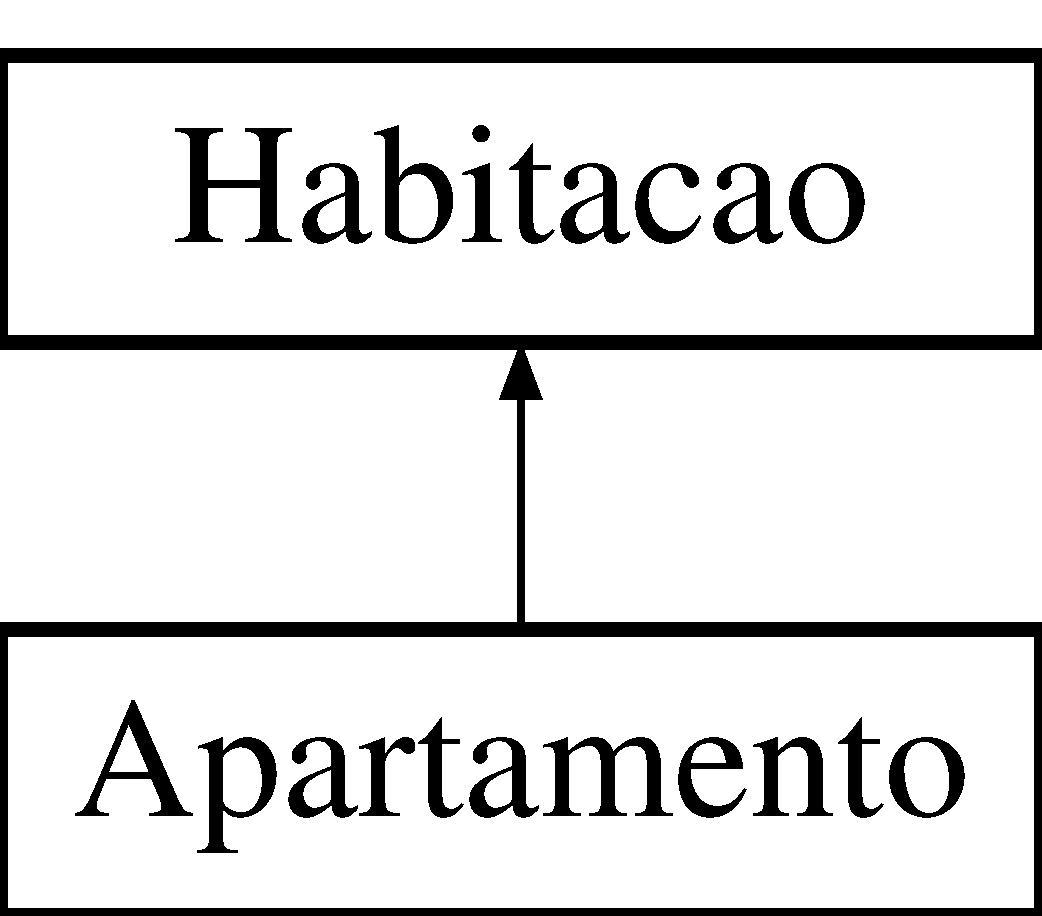
\includegraphics[height=2.000000cm]{class_apartamento}
\end{center}
\end{figure}
\subsection*{Public Member Functions}
\begin{DoxyCompactItemize}
\item 
\hyperlink{class_apartamento_ae5b9a8701fd002ea97962d4e7b3ace87}{Apartamento} (string morada, int area\+Habitacao, int tipologia, int piso)
\begin{DoxyCompactList}\small\item\em Função que cria um apartamento. \end{DoxyCompactList}\item 
float \hyperlink{class_apartamento_a3626df5dabd6871c5f9fce39e8c70249}{mensalidade} () const 
\begin{DoxyCompactList}\small\item\em Função que calcula o valor da base mensal de condomínio. \end{DoxyCompactList}\item 
void \hyperlink{class_apartamento_a272ca1ae1ea5b3ea7bc28388b1b79887}{get\+Informacoes} () const 
\begin{DoxyCompactList}\small\item\em Função para obter as informações do apartamento. \end{DoxyCompactList}\item 
int \hyperlink{class_apartamento_a8f933db9b6eb43fc714246e30b4bcf24}{get\+Tipologia} () const 
\begin{DoxyCompactList}\small\item\em Função para obter a tipologia. \end{DoxyCompactList}\item 
int \hyperlink{class_apartamento_a63f2569f807dc98bb632b4830ed18af4}{get\+Piso} () const 
\begin{DoxyCompactList}\small\item\em Função para obter o piso. \end{DoxyCompactList}\item 
void \hyperlink{class_apartamento_a4d66d10fb8c13d78296df641a640a13b}{set\+Tipologia} (int tipologia)
\begin{DoxyCompactList}\small\item\em Função para atualizar a tipologia do apartamento. \end{DoxyCompactList}\item 
void \hyperlink{class_apartamento_af620ef11e65b67939773cf23bc9a2582}{set\+Piso} (int piso)
\begin{DoxyCompactList}\small\item\em Função para atualizar o piso do apartamento. \end{DoxyCompactList}\end{DoxyCompactItemize}


\subsection{Constructor \& Destructor Documentation}
\index{Apartamento@{Apartamento}!Apartamento@{Apartamento}}
\index{Apartamento@{Apartamento}!Apartamento@{Apartamento}}
\subsubsection[{Apartamento(string morada, int area\+Habitacao, int tipologia, int piso)}]{\setlength{\rightskip}{0pt plus 5cm}Apartamento\+::\+Apartamento (
\begin{DoxyParamCaption}
\item[{string}]{morada, }
\item[{int}]{area\+Habitacao, }
\item[{int}]{tipologia, }
\item[{int}]{piso}
\end{DoxyParamCaption}
)}\hypertarget{class_apartamento_ae5b9a8701fd002ea97962d4e7b3ace87}{}\label{class_apartamento_ae5b9a8701fd002ea97962d4e7b3ace87}


Função que cria um apartamento. 


\begin{DoxyParams}{Parameters}
{\em morada} & -\/ localização geográfica do apartamento. \\
\hline
{\em area\+Habitacao} & -\/ area habitacional. \\
\hline
{\em tipologia} & -\/ tipo de apartamento, em que 1 equivale a T1, 2 a T2, etc. ... \\
\hline
{\em piso} & -\/ andar do apartamento. \\
\hline
\end{DoxyParams}


\subsection{Member Function Documentation}
\index{Apartamento@{Apartamento}!get\+Informacoes@{get\+Informacoes}}
\index{get\+Informacoes@{get\+Informacoes}!Apartamento@{Apartamento}}
\subsubsection[{get\+Informacoes() const }]{\setlength{\rightskip}{0pt plus 5cm}void Apartamento\+::get\+Informacoes (
\begin{DoxyParamCaption}
{}
\end{DoxyParamCaption}
) const\hspace{0.3cm}{\ttfamily [virtual]}}\hypertarget{class_apartamento_a272ca1ae1ea5b3ea7bc28388b1b79887}{}\label{class_apartamento_a272ca1ae1ea5b3ea7bc28388b1b79887}


Função para obter as informações do apartamento. 

\begin{DoxyReturn}{Returns}
Retorna as informações do apartamento 
\end{DoxyReturn}


Reimplemented from \hyperlink{class_habitacao}{Habitacao}.

\index{Apartamento@{Apartamento}!get\+Piso@{get\+Piso}}
\index{get\+Piso@{get\+Piso}!Apartamento@{Apartamento}}
\subsubsection[{get\+Piso() const }]{\setlength{\rightskip}{0pt plus 5cm}int Apartamento\+::get\+Piso (
\begin{DoxyParamCaption}
{}
\end{DoxyParamCaption}
) const}\hypertarget{class_apartamento_a63f2569f807dc98bb632b4830ed18af4}{}\label{class_apartamento_a63f2569f807dc98bb632b4830ed18af4}


Função para obter o piso. 

\begin{DoxyReturn}{Returns}
Retorna o piso. 
\end{DoxyReturn}
\index{Apartamento@{Apartamento}!get\+Tipologia@{get\+Tipologia}}
\index{get\+Tipologia@{get\+Tipologia}!Apartamento@{Apartamento}}
\subsubsection[{get\+Tipologia() const }]{\setlength{\rightskip}{0pt plus 5cm}int Apartamento\+::get\+Tipologia (
\begin{DoxyParamCaption}
{}
\end{DoxyParamCaption}
) const}\hypertarget{class_apartamento_a8f933db9b6eb43fc714246e30b4bcf24}{}\label{class_apartamento_a8f933db9b6eb43fc714246e30b4bcf24}


Função para obter a tipologia. 

\begin{DoxyReturn}{Returns}
Retorna a tipologia. 
\end{DoxyReturn}
\index{Apartamento@{Apartamento}!mensalidade@{mensalidade}}
\index{mensalidade@{mensalidade}!Apartamento@{Apartamento}}
\subsubsection[{mensalidade() const }]{\setlength{\rightskip}{0pt plus 5cm}float Apartamento\+::mensalidade (
\begin{DoxyParamCaption}
{}
\end{DoxyParamCaption}
) const\hspace{0.3cm}{\ttfamily [virtual]}}\hypertarget{class_apartamento_a3626df5dabd6871c5f9fce39e8c70249}{}\label{class_apartamento_a3626df5dabd6871c5f9fce39e8c70249}


Função que calcula o valor da base mensal de condomínio. 

\begin{DoxyReturn}{Returns}
Retorna o valor da base mensal de condomínio. 
\end{DoxyReturn}


Reimplemented from \hyperlink{class_habitacao_a479d2307661c87b05242b86ba849fb6e}{Habitacao}.

\index{Apartamento@{Apartamento}!set\+Piso@{set\+Piso}}
\index{set\+Piso@{set\+Piso}!Apartamento@{Apartamento}}
\subsubsection[{set\+Piso(int piso)}]{\setlength{\rightskip}{0pt plus 5cm}void Apartamento\+::set\+Piso (
\begin{DoxyParamCaption}
\item[{int}]{piso}
\end{DoxyParamCaption}
)}\hypertarget{class_apartamento_af620ef11e65b67939773cf23bc9a2582}{}\label{class_apartamento_af620ef11e65b67939773cf23bc9a2582}


Função para atualizar o piso do apartamento. 


\begin{DoxyParams}{Parameters}
{\em piso} & -\/ Piso do apartamento. \\
\hline
\end{DoxyParams}
\index{Apartamento@{Apartamento}!set\+Tipologia@{set\+Tipologia}}
\index{set\+Tipologia@{set\+Tipologia}!Apartamento@{Apartamento}}
\subsubsection[{set\+Tipologia(int tipologia)}]{\setlength{\rightskip}{0pt plus 5cm}void Apartamento\+::set\+Tipologia (
\begin{DoxyParamCaption}
\item[{int}]{tipologia}
\end{DoxyParamCaption}
)}\hypertarget{class_apartamento_a4d66d10fb8c13d78296df641a640a13b}{}\label{class_apartamento_a4d66d10fb8c13d78296df641a640a13b}


Função para atualizar a tipologia do apartamento. 


\begin{DoxyParams}{Parameters}
{\em tipologia} & -\/ Tipologia do apartamento. \\
\hline
\end{DoxyParams}


The documentation for this class was generated from the following files\+:\begin{DoxyCompactItemize}
\item 
Apartamento.\+h\item 
Apartamento.\+cpp\end{DoxyCompactItemize}

\hypertarget{class_canalizacao}{}\section{Canalizacao Class Reference}
\label{class_canalizacao}\index{Canalizacao@{Canalizacao}}
Inheritance diagram for Canalizacao\+:\begin{figure}[H]
\begin{center}
\leavevmode
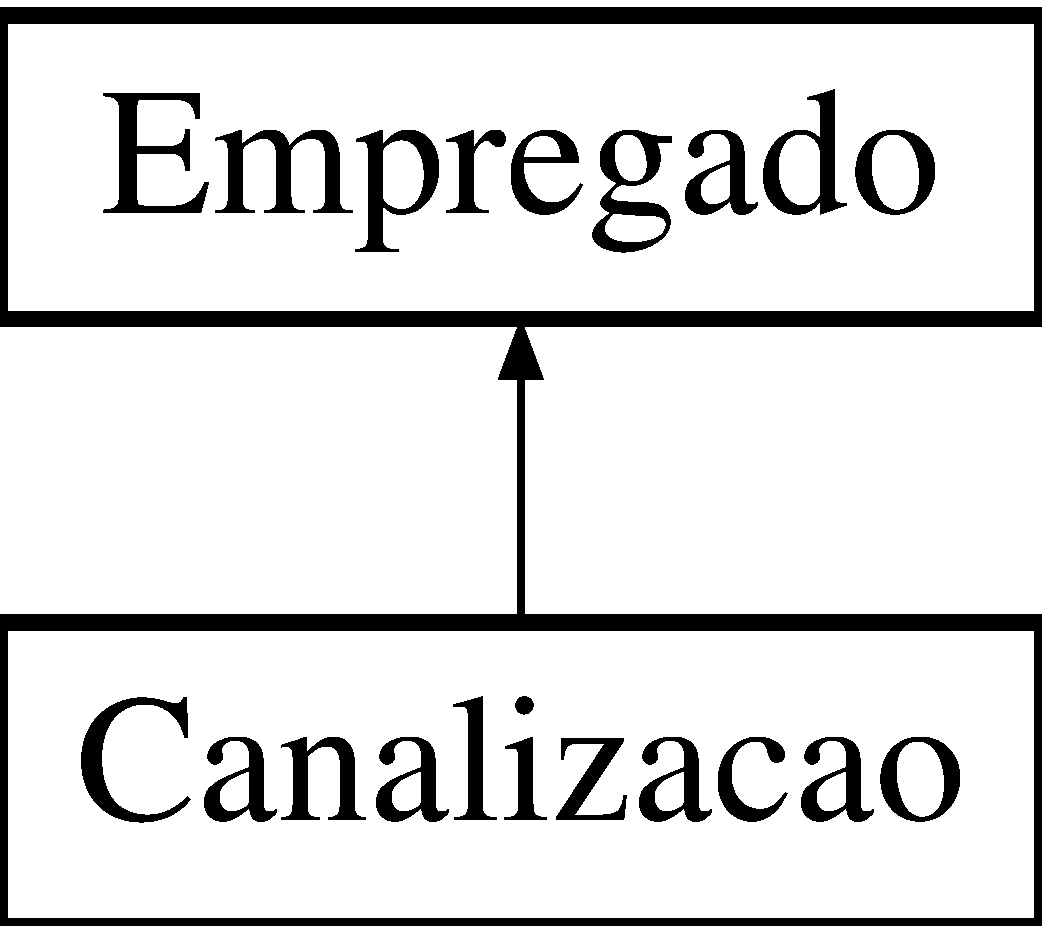
\includegraphics[height=2.000000cm]{class_canalizacao}
\end{center}
\end{figure}
\subsection*{Public Member Functions}
\begin{DoxyCompactItemize}
\item 
\hyperlink{class_canalizacao_ad547b610d50c91b0de57e30938971216}{Canalizacao} (string nome, int bi, int numero\+Telemovel, string email, string tipo, bool livre)
\begin{DoxyCompactList}\small\item\em Função que cria um empregado canalizador. \end{DoxyCompactList}\end{DoxyCompactItemize}


\subsection{Constructor \& Destructor Documentation}
\index{Canalizacao@{Canalizacao}!Canalizacao@{Canalizacao}}
\index{Canalizacao@{Canalizacao}!Canalizacao@{Canalizacao}}
\subsubsection[{Canalizacao(string nome, int bi, int numero\+Telemovel, string email, string tipo, bool livre)}]{\setlength{\rightskip}{0pt plus 5cm}Canalizacao\+::\+Canalizacao (
\begin{DoxyParamCaption}
\item[{string}]{nome, }
\item[{int}]{bi, }
\item[{int}]{numero\+Telemovel, }
\item[{string}]{email, }
\item[{string}]{tipo, }
\item[{bool}]{livre}
\end{DoxyParamCaption}
)}\hypertarget{class_canalizacao_ad547b610d50c91b0de57e30938971216}{}\label{class_canalizacao_ad547b610d50c91b0de57e30938971216}


Função que cria um empregado canalizador. 


\begin{DoxyParams}{Parameters}
{\em nome} & -\/ nome do empregado. \\
\hline
{\em bi} & -\/ número do bilhete de identidade. \\
\hline
{\em numero\+Telemovel} & -\/ número de telemóvel do empregado. \\
\hline
{\em email} & -\/ email do empregado. \\
\hline
{\em tipo} & -\/ o tipo deve ser \char`\"{}canalizador\char`\"{}, caso contrário é lançada uma exceção. \\
\hline
{\em livre} & -\/ se for verdadeiro então o empregado está livre, caso contrário está ocupado. \\
\hline
\end{DoxyParams}


The documentation for this class was generated from the following files\+:\begin{DoxyCompactItemize}
\item 
Canalizacao.\+h\item 
Canalizacao.\+cpp\end{DoxyCompactItemize}

\hypertarget{class_cliente}{}\section{Cliente Class Reference}
\label{class_cliente}\index{Cliente@{Cliente}}
\subsection*{Public Member Functions}
\begin{DoxyCompactItemize}
\item 
\hyperlink{class_cliente_a9c7edf7c69561bcb1170aa51ea09f0ee}{Cliente} (string nome, int bi, int numero\+Telemovel, string email, vector$<$ \hyperlink{class_habitacao}{Habitacao} $\ast$ $>$ habitacoes)
\begin{DoxyCompactList}\small\item\em Função que cria um cliente. \end{DoxyCompactList}\item 
int \hyperlink{class_cliente_a0ceeca7c7fd8910a7cd169b97cec7825}{existe\+Habitacao} (\hyperlink{class_habitacao}{Habitacao} $\ast$habitacao)
\begin{DoxyCompactList}\small\item\em Verifica se uma dada habitação existe nas habitações do cliente. \end{DoxyCompactList}\item 
int \hyperlink{class_cliente_a5e5c3a99a6b1941e481072240323a878}{adiciona\+Habitacao} (\hyperlink{class_habitacao}{Habitacao} $\ast$habitacao)
\begin{DoxyCompactList}\small\item\em Torna o cliente proprietário de uma dada habitação. \end{DoxyCompactList}\item 
int \hyperlink{class_cliente_af50893954314bc62ee0cef46e33bbb60}{remove\+Habitacao} (\hyperlink{class_habitacao}{Habitacao} $\ast$habitacao)
\begin{DoxyCompactList}\small\item\em Remove uma habitação das habitações do cliente. \end{DoxyCompactList}\item 
vector$<$ \hyperlink{class_habitacao}{Habitacao} $\ast$ $>$ \hyperlink{class_cliente_a6625c1bb73828bcaa067f41b7590408f}{get\+Habitacoes} () const 
\begin{DoxyCompactList}\small\item\em Função para obter as habitações do cliente. \end{DoxyCompactList}\item 
int \hyperlink{class_cliente_a800f49dc0761b67a61e563ca9a1478a7}{get\+BI} () const 
\begin{DoxyCompactList}\small\item\em Função para obter o número do bilhete de identidade do cliente. \end{DoxyCompactList}\item 
string \hyperlink{class_cliente_a0325de899469e2fed48ffda2b5b291cf}{get\+Nome} () const 
\begin{DoxyCompactList}\small\item\em Função para obter o nome do cliente. \end{DoxyCompactList}\item 
int \hyperlink{class_cliente_afce876126c623cc00e3c352830eba54c}{get\+Numero\+Telemovel} () const 
\begin{DoxyCompactList}\small\item\em Função para obter o número de telemóvel do cliente. \end{DoxyCompactList}\item 
string \hyperlink{class_cliente_a47c30bc1bd543033fa81ffe25e043e91}{get\+Email} () const 
\begin{DoxyCompactList}\small\item\em Função para obter o email do cliente. \end{DoxyCompactList}\item 
void \hyperlink{class_cliente_a383af20fa7ace06d4f04fe26e82e0ca2}{set\+Nome} (string nome)
\begin{DoxyCompactList}\small\item\em Função para atualizar o nome do cliente. \end{DoxyCompactList}\item 
void \hyperlink{class_cliente_a94b552224f9bb3b3189e2c92282f311f}{set\+BI} (int bi)
\begin{DoxyCompactList}\small\item\em Função para atualizar o BI do cliente. \end{DoxyCompactList}\item 
void \hyperlink{class_cliente_aa82126e31c6e41f79e0063125c80f77c}{set\+Numero\+Telemovel} (int numero\+Telemovel)
\begin{DoxyCompactList}\small\item\em Função para atualizar o número de telemóvel do cliente. \end{DoxyCompactList}\item 
void \hyperlink{class_cliente_a2c44b0f11f5d58b3f5b793a073ed1ac9}{set\+Email} (string email)
\begin{DoxyCompactList}\small\item\em Função para atualizar o email do cliente. \end{DoxyCompactList}\item 
bool \hyperlink{class_cliente_a1d84706fef989238713cf6efe3824696}{operator==} (const \hyperlink{class_cliente}{Cliente} \&cliente)
\begin{DoxyCompactList}\small\item\em Operador para verificar se dois clientes são o mesmo. \end{DoxyCompactList}\item 
bool \hyperlink{class_cliente_a627763ca5d6df1955d3449a402b118b6}{operator$<$} (const \hyperlink{class_cliente}{Cliente} \&cliente)
\begin{DoxyCompactList}\small\item\em Um cliente é menor que outro caso o seu nome seja alfabeticamente menor. \end{DoxyCompactList}\end{DoxyCompactItemize}


\subsection{Constructor \& Destructor Documentation}
\index{Cliente@{Cliente}!Cliente@{Cliente}}
\index{Cliente@{Cliente}!Cliente@{Cliente}}
\subsubsection[{Cliente(string nome, int bi, int numero\+Telemovel, string email, vector$<$ Habitacao $\ast$ $>$ habitacoes)}]{\setlength{\rightskip}{0pt plus 5cm}Cliente\+::\+Cliente (
\begin{DoxyParamCaption}
\item[{string}]{nome, }
\item[{int}]{bi, }
\item[{int}]{numero\+Telemovel, }
\item[{string}]{email, }
\item[{vector$<$ {\bf Habitacao} $\ast$ $>$}]{habitacoes}
\end{DoxyParamCaption}
)}\hypertarget{class_cliente_a9c7edf7c69561bcb1170aa51ea09f0ee}{}\label{class_cliente_a9c7edf7c69561bcb1170aa51ea09f0ee}


Função que cria um cliente. 


\begin{DoxyParams}{Parameters}
{\em nome} & -\/ nome do cliente. \\
\hline
{\em bi} & -\/ número do bilhete de identidade. \\
\hline
{\em habitacoes} & -\/ habitações das quais o cliente é proprietário. \\
\hline
\end{DoxyParams}


\subsection{Member Function Documentation}
\index{Cliente@{Cliente}!adiciona\+Habitacao@{adiciona\+Habitacao}}
\index{adiciona\+Habitacao@{adiciona\+Habitacao}!Cliente@{Cliente}}
\subsubsection[{adiciona\+Habitacao(\+Habitacao $\ast$habitacao)}]{\setlength{\rightskip}{0pt plus 5cm}int Cliente\+::adiciona\+Habitacao (
\begin{DoxyParamCaption}
\item[{{\bf Habitacao} $\ast$}]{habitacao}
\end{DoxyParamCaption}
)}\hypertarget{class_cliente_a5e5c3a99a6b1941e481072240323a878}{}\label{class_cliente_a5e5c3a99a6b1941e481072240323a878}


Torna o cliente proprietário de uma dada habitação. 


\begin{DoxyParams}{Parameters}
{\em habitacao} & -\/ habitação que se pretende adicionar. \\
\hline
\end{DoxyParams}
\begin{DoxyReturn}{Returns}
Retorna 0 em caso de sucesso. 
\end{DoxyReturn}
\index{Cliente@{Cliente}!existe\+Habitacao@{existe\+Habitacao}}
\index{existe\+Habitacao@{existe\+Habitacao}!Cliente@{Cliente}}
\subsubsection[{existe\+Habitacao(\+Habitacao $\ast$habitacao)}]{\setlength{\rightskip}{0pt plus 5cm}int Cliente\+::existe\+Habitacao (
\begin{DoxyParamCaption}
\item[{{\bf Habitacao} $\ast$}]{habitacao}
\end{DoxyParamCaption}
)}\hypertarget{class_cliente_a0ceeca7c7fd8910a7cd169b97cec7825}{}\label{class_cliente_a0ceeca7c7fd8910a7cd169b97cec7825}


Verifica se uma dada habitação existe nas habitações do cliente. 


\begin{DoxyParams}{Parameters}
{\em habitacao} & -\/ habitação que se pretende procurar. \\
\hline
\end{DoxyParams}
\begin{DoxyReturn}{Returns}
Retorna a posição da habitação que pertence às habitações do cliente ou -\/1 caso não exista. 
\end{DoxyReturn}
\index{Cliente@{Cliente}!get\+BI@{get\+BI}}
\index{get\+BI@{get\+BI}!Cliente@{Cliente}}
\subsubsection[{get\+B\+I() const }]{\setlength{\rightskip}{0pt plus 5cm}int Cliente\+::get\+BI (
\begin{DoxyParamCaption}
{}
\end{DoxyParamCaption}
) const}\hypertarget{class_cliente_a800f49dc0761b67a61e563ca9a1478a7}{}\label{class_cliente_a800f49dc0761b67a61e563ca9a1478a7}


Função para obter o número do bilhete de identidade do cliente. 

\begin{DoxyReturn}{Returns}
Retorna o número do bilhete de identidade do cliente. 
\end{DoxyReturn}
\index{Cliente@{Cliente}!get\+Email@{get\+Email}}
\index{get\+Email@{get\+Email}!Cliente@{Cliente}}
\subsubsection[{get\+Email() const }]{\setlength{\rightskip}{0pt plus 5cm}string Cliente\+::get\+Email (
\begin{DoxyParamCaption}
{}
\end{DoxyParamCaption}
) const}\hypertarget{class_cliente_a47c30bc1bd543033fa81ffe25e043e91}{}\label{class_cliente_a47c30bc1bd543033fa81ffe25e043e91}


Função para obter o email do cliente. 

\begin{DoxyReturn}{Returns}
Retorna o email do cliente. 
\end{DoxyReturn}
\index{Cliente@{Cliente}!get\+Habitacoes@{get\+Habitacoes}}
\index{get\+Habitacoes@{get\+Habitacoes}!Cliente@{Cliente}}
\subsubsection[{get\+Habitacoes() const }]{\setlength{\rightskip}{0pt plus 5cm}vector$<$ {\bf Habitacao} $\ast$ $>$ Cliente\+::get\+Habitacoes (
\begin{DoxyParamCaption}
{}
\end{DoxyParamCaption}
) const}\hypertarget{class_cliente_a6625c1bb73828bcaa067f41b7590408f}{}\label{class_cliente_a6625c1bb73828bcaa067f41b7590408f}


Função para obter as habitações do cliente. 

\begin{DoxyReturn}{Returns}
Retorna as habitações do cliente. 
\end{DoxyReturn}
\index{Cliente@{Cliente}!get\+Nome@{get\+Nome}}
\index{get\+Nome@{get\+Nome}!Cliente@{Cliente}}
\subsubsection[{get\+Nome() const }]{\setlength{\rightskip}{0pt plus 5cm}string Cliente\+::get\+Nome (
\begin{DoxyParamCaption}
{}
\end{DoxyParamCaption}
) const}\hypertarget{class_cliente_a0325de899469e2fed48ffda2b5b291cf}{}\label{class_cliente_a0325de899469e2fed48ffda2b5b291cf}


Função para obter o nome do cliente. 

\begin{DoxyReturn}{Returns}
Retorna o nome do cliente. 
\end{DoxyReturn}
\index{Cliente@{Cliente}!get\+Numero\+Telemovel@{get\+Numero\+Telemovel}}
\index{get\+Numero\+Telemovel@{get\+Numero\+Telemovel}!Cliente@{Cliente}}
\subsubsection[{get\+Numero\+Telemovel() const }]{\setlength{\rightskip}{0pt plus 5cm}int Cliente\+::get\+Numero\+Telemovel (
\begin{DoxyParamCaption}
{}
\end{DoxyParamCaption}
) const}\hypertarget{class_cliente_afce876126c623cc00e3c352830eba54c}{}\label{class_cliente_afce876126c623cc00e3c352830eba54c}


Função para obter o número de telemóvel do cliente. 

\begin{DoxyReturn}{Returns}
Retorna o número de telemóvel do cliente. 
\end{DoxyReturn}
\index{Cliente@{Cliente}!operator$<$@{operator$<$}}
\index{operator$<$@{operator$<$}!Cliente@{Cliente}}
\subsubsection[{operator$<$(const Cliente \&cliente)}]{\setlength{\rightskip}{0pt plus 5cm}bool Cliente\+::operator$<$ (
\begin{DoxyParamCaption}
\item[{const {\bf Cliente} \&}]{cliente}
\end{DoxyParamCaption}
)}\hypertarget{class_cliente_a627763ca5d6df1955d3449a402b118b6}{}\label{class_cliente_a627763ca5d6df1955d3449a402b118b6}


Um cliente é menor que outro caso o seu nome seja alfabeticamente menor. 


\begin{DoxyParams}{Parameters}
{\em cliente} & -\/ cliente externo com o qual vai ser comparado o cliente. \\
\hline
\end{DoxyParams}
\begin{DoxyReturn}{Returns}
Retorna verdade caso o cliente externo seja maior alfabeticamente que o cliente e falso caso contrário. 
\end{DoxyReturn}
\index{Cliente@{Cliente}!operator==@{operator==}}
\index{operator==@{operator==}!Cliente@{Cliente}}
\subsubsection[{operator==(const Cliente \&cliente)}]{\setlength{\rightskip}{0pt plus 5cm}bool Cliente\+::operator== (
\begin{DoxyParamCaption}
\item[{const {\bf Cliente} \&}]{cliente}
\end{DoxyParamCaption}
)}\hypertarget{class_cliente_a1d84706fef989238713cf6efe3824696}{}\label{class_cliente_a1d84706fef989238713cf6efe3824696}


Operador para verificar se dois clientes são o mesmo. 


\begin{DoxyParams}{Parameters}
{\em cliente} & -\/ cliente externo com o qual vai ser comparado o cliente. \\
\hline
\end{DoxyParams}
\begin{DoxyReturn}{Returns}
Retorna verdade caso os clientes sejam o mesmo e falso caso contrário. 
\end{DoxyReturn}
\index{Cliente@{Cliente}!remove\+Habitacao@{remove\+Habitacao}}
\index{remove\+Habitacao@{remove\+Habitacao}!Cliente@{Cliente}}
\subsubsection[{remove\+Habitacao(\+Habitacao $\ast$habitacao)}]{\setlength{\rightskip}{0pt plus 5cm}int Cliente\+::remove\+Habitacao (
\begin{DoxyParamCaption}
\item[{{\bf Habitacao} $\ast$}]{habitacao}
\end{DoxyParamCaption}
)}\hypertarget{class_cliente_af50893954314bc62ee0cef46e33bbb60}{}\label{class_cliente_af50893954314bc62ee0cef46e33bbb60}


Remove uma habitação das habitações do cliente. 


\begin{DoxyParams}{Parameters}
{\em habitacao} & -\/ habitação que se pretende remover. \\
\hline
\end{DoxyParams}
\begin{DoxyReturn}{Returns}
Retorna 0 em caso de sucesso. 
\end{DoxyReturn}
\index{Cliente@{Cliente}!set\+BI@{set\+BI}}
\index{set\+BI@{set\+BI}!Cliente@{Cliente}}
\subsubsection[{set\+B\+I(int bi)}]{\setlength{\rightskip}{0pt plus 5cm}void Cliente\+::set\+BI (
\begin{DoxyParamCaption}
\item[{int}]{bi}
\end{DoxyParamCaption}
)}\hypertarget{class_cliente_a94b552224f9bb3b3189e2c92282f311f}{}\label{class_cliente_a94b552224f9bb3b3189e2c92282f311f}


Função para atualizar o BI do cliente. 


\begin{DoxyParams}{Parameters}
{\em bi} & -\/ Novo BI do cliente. \\
\hline
\end{DoxyParams}
\index{Cliente@{Cliente}!set\+Email@{set\+Email}}
\index{set\+Email@{set\+Email}!Cliente@{Cliente}}
\subsubsection[{set\+Email(string email)}]{\setlength{\rightskip}{0pt plus 5cm}void Cliente\+::set\+Email (
\begin{DoxyParamCaption}
\item[{string}]{email}
\end{DoxyParamCaption}
)}\hypertarget{class_cliente_a2c44b0f11f5d58b3f5b793a073ed1ac9}{}\label{class_cliente_a2c44b0f11f5d58b3f5b793a073ed1ac9}


Função para atualizar o email do cliente. 


\begin{DoxyParams}{Parameters}
{\em email} & -\/ Novo email do cliente. \\
\hline
\end{DoxyParams}
\index{Cliente@{Cliente}!set\+Nome@{set\+Nome}}
\index{set\+Nome@{set\+Nome}!Cliente@{Cliente}}
\subsubsection[{set\+Nome(string nome)}]{\setlength{\rightskip}{0pt plus 5cm}void Cliente\+::set\+Nome (
\begin{DoxyParamCaption}
\item[{string}]{nome}
\end{DoxyParamCaption}
)}\hypertarget{class_cliente_a383af20fa7ace06d4f04fe26e82e0ca2}{}\label{class_cliente_a383af20fa7ace06d4f04fe26e82e0ca2}


Função para atualizar o nome do cliente. 


\begin{DoxyParams}{Parameters}
{\em nome} & -\/ Novo nome do cliente. \\
\hline
\end{DoxyParams}
\index{Cliente@{Cliente}!set\+Numero\+Telemovel@{set\+Numero\+Telemovel}}
\index{set\+Numero\+Telemovel@{set\+Numero\+Telemovel}!Cliente@{Cliente}}
\subsubsection[{set\+Numero\+Telemovel(int numero\+Telemovel)}]{\setlength{\rightskip}{0pt plus 5cm}void Cliente\+::set\+Numero\+Telemovel (
\begin{DoxyParamCaption}
\item[{int}]{numero\+Telemovel}
\end{DoxyParamCaption}
)}\hypertarget{class_cliente_aa82126e31c6e41f79e0063125c80f77c}{}\label{class_cliente_aa82126e31c6e41f79e0063125c80f77c}


Função para atualizar o número de telemóvel do cliente. 


\begin{DoxyParams}{Parameters}
{\em numero\+Telemovel} & -\/ Novo número de telemóvel do cliente. \\
\hline
\end{DoxyParams}


The documentation for this class was generated from the following files\+:\begin{DoxyCompactItemize}
\item 
Cliente.\+h\item 
Cliente.\+cpp\end{DoxyCompactItemize}

\hypertarget{class_condominio}{}\section{Condominio Class Reference}
\label{class_condominio}\index{Condominio@{Condominio}}
\subsection*{Public Member Functions}
\begin{DoxyCompactItemize}
\item 
\hyperlink{class_condominio_a69e71aaab401f7ff0a92ff0f45bdb751}{Condominio} (string designacao, int nif, int numero\+Telefone, string email, vector$<$ \hyperlink{class_cliente}{Cliente} $\ast$ $>$ clientes, \hyperlink{class_servico}{Servico} $\ast$servico, string localizacao)
\begin{DoxyCompactList}\small\item\em Função que cria um condominio. \end{DoxyCompactList}\item 
int \hyperlink{class_condominio_a08e2bf58344131ff357f2f7ed62a56fb}{existe\+Cliente} (\hyperlink{class_cliente}{Cliente} $\ast$cliente)
\begin{DoxyCompactList}\small\item\em Verifica se um dado cliente pertence ao condomínio. \end{DoxyCompactList}\item 
int \hyperlink{class_condominio_ae27a8bd9f2e1ad20b18dd34b4bd997d6}{adiciona\+Cliente} (\hyperlink{class_cliente}{Cliente} $\ast$cliente)
\begin{DoxyCompactList}\small\item\em Adiciona um cliente aos clientes do condomínio. \end{DoxyCompactList}\item 
int \hyperlink{class_condominio_ac62185f435dd9c3538a795aa7908beac}{remove\+Cliente} (\hyperlink{class_cliente}{Cliente} $\ast$cliente)
\begin{DoxyCompactList}\small\item\em Remove um dado cliente dos clientes do condomínio. \end{DoxyCompactList}\item 
float \hyperlink{class_condominio_a16747ea7d4e1b442b1985725f5a9aeab}{pagar\+Mensalidade} (\hyperlink{class_habitacao}{Habitacao} $\ast$habitacao) const 
\begin{DoxyCompactList}\small\item\em Função para efetuar o pagamento da base mensal de condomínio de uma habitação. \end{DoxyCompactList}\item 
\hyperlink{class_empregado}{Empregado} $\ast$ \hyperlink{class_condominio_a5eec0c5c3a1cb566332431939bcbcb56}{requisita\+Empregado} (string tipo)
\begin{DoxyCompactList}\small\item\em Requisita um empregado de um dado tipo.  -\/ tipo do empregado pretendido. \end{DoxyCompactList}\item 
int \hyperlink{class_condominio_adb5c91a9114dbc1c0f3c8c3e9f835152}{requisita\+Servico} (string tipo, \hyperlink{class_habitacao}{Habitacao} $\ast$habitacao)
\begin{DoxyCompactList}\small\item\em Requisita um serviço de um dado tipo. \end{DoxyCompactList}\item 
int \hyperlink{class_condominio_af2c2cdd83d43ea6641542efe01ff94b9}{fim\+Do\+Servico} (\hyperlink{class_empregado}{Empregado} $\ast$empregado)
\begin{DoxyCompactList}\small\item\em Coloca um empregado livre quando acaba de prestar um serviço. \end{DoxyCompactList}\item 
int \hyperlink{class_condominio_abfbd356bc26fde54dc40de2f9174f430}{consulta\+Cliente} (int cliente) const 
\begin{DoxyCompactList}\small\item\em Consulta dados de um dado cliente. \end{DoxyCompactList}\item 
int \hyperlink{class_condominio_a37df336e62f83189d9193f039e58935d}{get\+Id} () const 
\begin{DoxyCompactList}\small\item\em Função que retorna o identificador do condomínio. \end{DoxyCompactList}\item 
string \hyperlink{class_condominio_a1c9390d8d9fcfe834568d74041a49e04}{get\+Designacao} () const 
\begin{DoxyCompactList}\small\item\em Função para obter a designacao do condominio. \end{DoxyCompactList}\item 
int \hyperlink{class_condominio_a131891ab8b9ca504227ec3f9edcbc326}{get\+N\+IF} () const 
\begin{DoxyCompactList}\small\item\em Função para obter o N\+IF do condominio. \end{DoxyCompactList}\item 
int \hyperlink{class_condominio_adc7a4de5ad8ace80c0290fff0619f22d}{get\+Numero\+Telefone} () const 
\begin{DoxyCompactList}\small\item\em Função para obter o número de telefone do condominio. \end{DoxyCompactList}\item 
string \hyperlink{class_condominio_adc4a6fa8a9fcb43a65226b722b7929d0}{get\+Email} () const 
\begin{DoxyCompactList}\small\item\em Função para obter o email do condominio. \end{DoxyCompactList}\item 
string \hyperlink{class_condominio_a9404521b87cc71622544fe8ecc9c28fb}{get\+Localizacao} () const 
\begin{DoxyCompactList}\small\item\em Função para obter a localização do condomínio. \end{DoxyCompactList}\item 
vector$<$ \hyperlink{class_cliente}{Cliente} $\ast$ $>$ \hyperlink{class_condominio_a6a9100e8a8a48847785f4c4b108ab8db}{get\+Clientes} () const 
\begin{DoxyCompactList}\small\item\em Função para obter os clientes do condomínio. \end{DoxyCompactList}\item 
\hyperlink{class_servico}{Servico} $\ast$ \hyperlink{class_condominio_abb987c983caf8468935773b00505a5e2}{get\+Servico} () const 
\begin{DoxyCompactList}\small\item\em Função para obter a empresa de serviços. \end{DoxyCompactList}\item 
int \hyperlink{class_condominio_a81756f3ac4301c65deade4c520ea6ae1}{get\+Num\+Habs} () const 
\begin{DoxyCompactList}\small\item\em Função para obter o número de habitações do condomínio. \end{DoxyCompactList}\item 
int \hyperlink{class_condominio_a47e2e368a9e643017cad7a2e30a4c087}{get\+Num\+Vivendas} () const 
\begin{DoxyCompactList}\small\item\em Função para obter o número de vivendas do condomínio. \end{DoxyCompactList}\item 
void \hyperlink{class_condominio_a54e452fd5905ec95a028cd2dfefbc437}{set\+Designacao} (string designacao)
\begin{DoxyCompactList}\small\item\em Função para atualizar a designacao do condomínio. \end{DoxyCompactList}\item 
void \hyperlink{class_condominio_a89d828306fcbcc0df34d52e07b7e9bb7}{set\+N\+IF} (int nif)
\begin{DoxyCompactList}\small\item\em Função para atualizar o N\+IF do condomínio. \end{DoxyCompactList}\item 
void \hyperlink{class_condominio_a7f454a535fe1ebc3ab244415d963b719}{set\+Numero\+Telefone} (int numero\+Telefone)
\begin{DoxyCompactList}\small\item\em Função para atualizar o número de telefone do condomínio. \end{DoxyCompactList}\item 
void \hyperlink{class_condominio_ae0521eb8186f3c4000cc8c0fa6d4b762}{set\+Email} (string email)
\begin{DoxyCompactList}\small\item\em Função para atualizar o email do condomínio. \end{DoxyCompactList}\item 
void \hyperlink{class_condominio_ae87fcb0812e926dbdf6609f3359b9df9}{set\+Localizacao} (string localizacao)
\begin{DoxyCompactList}\small\item\em Função para atualizar a localização do condomínio. \end{DoxyCompactList}\item 
bool \hyperlink{class_condominio_ad42a7789ca5fc636ff97018f93426055}{operator==} (const \hyperlink{class_condominio}{Condominio} \&cond) const 
\begin{DoxyCompactList}\small\item\em Operador para verificar se dois condomínios são o mesmo. \end{DoxyCompactList}\item 
bool \hyperlink{class_condominio_a522f22fe4aedc504dab8728e73945777}{operator$<$} (const \hyperlink{class_condominio}{Condominio} \&cond2) const 
\begin{DoxyCompactList}\small\item\em Operador para verificar se um condominio é menor que outro. \end{DoxyCompactList}\end{DoxyCompactItemize}
\subsection*{Static Public Attributes}
\begin{DoxyCompactItemize}
\item 
static int {\bfseries last\+Id} = 0\hypertarget{class_condominio_ad6d8cc37886212f5dbf8260c25a94961}{}\label{class_condominio_ad6d8cc37886212f5dbf8260c25a94961}

\end{DoxyCompactItemize}


\subsection{Constructor \& Destructor Documentation}
\index{Condominio@{Condominio}!Condominio@{Condominio}}
\index{Condominio@{Condominio}!Condominio@{Condominio}}
\subsubsection[{Condominio(string designacao, int nif, int numero\+Telefone, string email, vector$<$ Cliente $\ast$ $>$ clientes, Servico $\ast$servico, string localizacao)}]{\setlength{\rightskip}{0pt plus 5cm}Condominio\+::\+Condominio (
\begin{DoxyParamCaption}
\item[{string}]{designacao, }
\item[{int}]{nif, }
\item[{int}]{numero\+Telefone, }
\item[{string}]{email, }
\item[{vector$<$ {\bf Cliente} $\ast$ $>$}]{clientes, }
\item[{{\bf Servico} $\ast$}]{servico, }
\item[{string}]{localizacao}
\end{DoxyParamCaption}
)}\hypertarget{class_condominio_a69e71aaab401f7ff0a92ff0f45bdb751}{}\label{class_condominio_a69e71aaab401f7ff0a92ff0f45bdb751}


Função que cria um condominio. 


\begin{DoxyParams}{Parameters}
{\em designacao} & -\/ nome do condomínio. \\
\hline
{\em nif} & -\/ número de identificação fiscal do condomínio. \\
\hline
{\em numero\+Telefone} & -\/ número de telefone do condomínio. \\
\hline
{\em email} & -\/ email do condomínio. \\
\hline
{\em clientes} & -\/ clientes do condomínio. \\
\hline
{\em serviço} & -\/ empresa de serviços. \\
\hline
\end{DoxyParams}


\subsection{Member Function Documentation}
\index{Condominio@{Condominio}!adiciona\+Cliente@{adiciona\+Cliente}}
\index{adiciona\+Cliente@{adiciona\+Cliente}!Condominio@{Condominio}}
\subsubsection[{adiciona\+Cliente(\+Cliente $\ast$cliente)}]{\setlength{\rightskip}{0pt plus 5cm}int Condominio\+::adiciona\+Cliente (
\begin{DoxyParamCaption}
\item[{{\bf Cliente} $\ast$}]{cliente}
\end{DoxyParamCaption}
)}\hypertarget{class_condominio_ae27a8bd9f2e1ad20b18dd34b4bd997d6}{}\label{class_condominio_ae27a8bd9f2e1ad20b18dd34b4bd997d6}


Adiciona um cliente aos clientes do condomínio. 


\begin{DoxyParams}{Parameters}
{\em cliente} & -\/ cliente que se quer adicionar aos clientes do condomínio. \\
\hline
\end{DoxyParams}
\begin{DoxyReturn}{Returns}
Retorna 0 em caso de sucesso. 
\end{DoxyReturn}
\index{Condominio@{Condominio}!consulta\+Cliente@{consulta\+Cliente}}
\index{consulta\+Cliente@{consulta\+Cliente}!Condominio@{Condominio}}
\subsubsection[{consulta\+Cliente(int cliente) const }]{\setlength{\rightskip}{0pt plus 5cm}int Condominio\+::consulta\+Cliente (
\begin{DoxyParamCaption}
\item[{int}]{cliente}
\end{DoxyParamCaption}
) const}\hypertarget{class_condominio_abfbd356bc26fde54dc40de2f9174f430}{}\label{class_condominio_abfbd356bc26fde54dc40de2f9174f430}


Consulta dados de um dado cliente. 


\begin{DoxyParams}{Parameters}
{\em cliente} & -\/ bi do cliente que vai ser procurado. \\
\hline
\end{DoxyParams}
\begin{DoxyReturn}{Returns}
Retorna 0 em caso de sucesso. 
\end{DoxyReturn}
\index{Condominio@{Condominio}!existe\+Cliente@{existe\+Cliente}}
\index{existe\+Cliente@{existe\+Cliente}!Condominio@{Condominio}}
\subsubsection[{existe\+Cliente(\+Cliente $\ast$cliente)}]{\setlength{\rightskip}{0pt plus 5cm}int Condominio\+::existe\+Cliente (
\begin{DoxyParamCaption}
\item[{{\bf Cliente} $\ast$}]{cliente}
\end{DoxyParamCaption}
)}\hypertarget{class_condominio_a08e2bf58344131ff357f2f7ed62a56fb}{}\label{class_condominio_a08e2bf58344131ff357f2f7ed62a56fb}


Verifica se um dado cliente pertence ao condomínio. 


\begin{DoxyParams}{Parameters}
{\em cliente} & -\/ cliente que se pretende procurar. \\
\hline
\end{DoxyParams}
\begin{DoxyReturn}{Returns}
Retorna a posição do cliente que pertence ao condomínio ou -\/1 caso o cliente não exista. 
\end{DoxyReturn}
\index{Condominio@{Condominio}!fim\+Do\+Servico@{fim\+Do\+Servico}}
\index{fim\+Do\+Servico@{fim\+Do\+Servico}!Condominio@{Condominio}}
\subsubsection[{fim\+Do\+Servico(\+Empregado $\ast$empregado)}]{\setlength{\rightskip}{0pt plus 5cm}int Condominio\+::fim\+Do\+Servico (
\begin{DoxyParamCaption}
\item[{{\bf Empregado} $\ast$}]{empregado}
\end{DoxyParamCaption}
)}\hypertarget{class_condominio_af2c2cdd83d43ea6641542efe01ff94b9}{}\label{class_condominio_af2c2cdd83d43ea6641542efe01ff94b9}


Coloca um empregado livre quando acaba de prestar um serviço. 


\begin{DoxyParams}{Parameters}
{\em empregado} & -\/ empregado que terminou o serviço. \\
\hline
\end{DoxyParams}
\begin{DoxyReturn}{Returns}
Retorna 0 em caso de sucesso e -\/1 caso contrário. 
\end{DoxyReturn}
\index{Condominio@{Condominio}!get\+Clientes@{get\+Clientes}}
\index{get\+Clientes@{get\+Clientes}!Condominio@{Condominio}}
\subsubsection[{get\+Clientes() const }]{\setlength{\rightskip}{0pt plus 5cm}vector$<$ {\bf Cliente} $\ast$ $>$ Condominio\+::get\+Clientes (
\begin{DoxyParamCaption}
{}
\end{DoxyParamCaption}
) const}\hypertarget{class_condominio_a6a9100e8a8a48847785f4c4b108ab8db}{}\label{class_condominio_a6a9100e8a8a48847785f4c4b108ab8db}


Função para obter os clientes do condomínio. 

\begin{DoxyReturn}{Returns}
Retorna os clientes do condomínio. 
\end{DoxyReturn}
\index{Condominio@{Condominio}!get\+Designacao@{get\+Designacao}}
\index{get\+Designacao@{get\+Designacao}!Condominio@{Condominio}}
\subsubsection[{get\+Designacao() const }]{\setlength{\rightskip}{0pt plus 5cm}string Condominio\+::get\+Designacao (
\begin{DoxyParamCaption}
{}
\end{DoxyParamCaption}
) const}\hypertarget{class_condominio_a1c9390d8d9fcfe834568d74041a49e04}{}\label{class_condominio_a1c9390d8d9fcfe834568d74041a49e04}


Função para obter a designacao do condominio. 

\begin{DoxyReturn}{Returns}
Retorna a designacao do condominio. 
\end{DoxyReturn}
\index{Condominio@{Condominio}!get\+Email@{get\+Email}}
\index{get\+Email@{get\+Email}!Condominio@{Condominio}}
\subsubsection[{get\+Email() const }]{\setlength{\rightskip}{0pt plus 5cm}string Condominio\+::get\+Email (
\begin{DoxyParamCaption}
{}
\end{DoxyParamCaption}
) const}\hypertarget{class_condominio_adc4a6fa8a9fcb43a65226b722b7929d0}{}\label{class_condominio_adc4a6fa8a9fcb43a65226b722b7929d0}


Função para obter o email do condominio. 

\begin{DoxyReturn}{Returns}
Retorna o email do condominio. 
\end{DoxyReturn}
\index{Condominio@{Condominio}!get\+Id@{get\+Id}}
\index{get\+Id@{get\+Id}!Condominio@{Condominio}}
\subsubsection[{get\+Id() const }]{\setlength{\rightskip}{0pt plus 5cm}int Condominio\+::get\+Id (
\begin{DoxyParamCaption}
{}
\end{DoxyParamCaption}
) const}\hypertarget{class_condominio_a37df336e62f83189d9193f039e58935d}{}\label{class_condominio_a37df336e62f83189d9193f039e58935d}


Função que retorna o identificador do condomínio. 

\begin{DoxyReturn}{Returns}
Retorna o identificador do condomínio. 
\end{DoxyReturn}
\index{Condominio@{Condominio}!get\+Localizacao@{get\+Localizacao}}
\index{get\+Localizacao@{get\+Localizacao}!Condominio@{Condominio}}
\subsubsection[{get\+Localizacao() const }]{\setlength{\rightskip}{0pt plus 5cm}string Condominio\+::get\+Localizacao (
\begin{DoxyParamCaption}
{}
\end{DoxyParamCaption}
) const}\hypertarget{class_condominio_a9404521b87cc71622544fe8ecc9c28fb}{}\label{class_condominio_a9404521b87cc71622544fe8ecc9c28fb}


Função para obter a localização do condomínio. 

\begin{DoxyReturn}{Returns}
Retorna a localização do condomínio. 
\end{DoxyReturn}
\index{Condominio@{Condominio}!get\+N\+IF@{get\+N\+IF}}
\index{get\+N\+IF@{get\+N\+IF}!Condominio@{Condominio}}
\subsubsection[{get\+N\+I\+F() const }]{\setlength{\rightskip}{0pt plus 5cm}int Condominio\+::get\+N\+IF (
\begin{DoxyParamCaption}
{}
\end{DoxyParamCaption}
) const}\hypertarget{class_condominio_a131891ab8b9ca504227ec3f9edcbc326}{}\label{class_condominio_a131891ab8b9ca504227ec3f9edcbc326}


Função para obter o N\+IF do condominio. 

\begin{DoxyReturn}{Returns}
Retorna o N\+IF do condominio. 
\end{DoxyReturn}
\index{Condominio@{Condominio}!get\+Numero\+Telefone@{get\+Numero\+Telefone}}
\index{get\+Numero\+Telefone@{get\+Numero\+Telefone}!Condominio@{Condominio}}
\subsubsection[{get\+Numero\+Telefone() const }]{\setlength{\rightskip}{0pt plus 5cm}int Condominio\+::get\+Numero\+Telefone (
\begin{DoxyParamCaption}
{}
\end{DoxyParamCaption}
) const}\hypertarget{class_condominio_adc7a4de5ad8ace80c0290fff0619f22d}{}\label{class_condominio_adc7a4de5ad8ace80c0290fff0619f22d}


Função para obter o número de telefone do condominio. 

\begin{DoxyReturn}{Returns}
Retorna o número de telefone do condominio. 
\end{DoxyReturn}
\index{Condominio@{Condominio}!get\+Num\+Habs@{get\+Num\+Habs}}
\index{get\+Num\+Habs@{get\+Num\+Habs}!Condominio@{Condominio}}
\subsubsection[{get\+Num\+Habs() const }]{\setlength{\rightskip}{0pt plus 5cm}int Condominio\+::get\+Num\+Habs (
\begin{DoxyParamCaption}
{}
\end{DoxyParamCaption}
) const}\hypertarget{class_condominio_a81756f3ac4301c65deade4c520ea6ae1}{}\label{class_condominio_a81756f3ac4301c65deade4c520ea6ae1}


Função para obter o número de habitações do condomínio. 

\begin{DoxyReturn}{Returns}
Retorna o número de habitações do condomínio. 
\end{DoxyReturn}
\index{Condominio@{Condominio}!get\+Num\+Vivendas@{get\+Num\+Vivendas}}
\index{get\+Num\+Vivendas@{get\+Num\+Vivendas}!Condominio@{Condominio}}
\subsubsection[{get\+Num\+Vivendas() const }]{\setlength{\rightskip}{0pt plus 5cm}int Condominio\+::get\+Num\+Vivendas (
\begin{DoxyParamCaption}
{}
\end{DoxyParamCaption}
) const}\hypertarget{class_condominio_a47e2e368a9e643017cad7a2e30a4c087}{}\label{class_condominio_a47e2e368a9e643017cad7a2e30a4c087}


Função para obter o número de vivendas do condomínio. 

\begin{DoxyReturn}{Returns}
Retorna o número de vivendas do condomínio. 
\end{DoxyReturn}
\index{Condominio@{Condominio}!get\+Servico@{get\+Servico}}
\index{get\+Servico@{get\+Servico}!Condominio@{Condominio}}
\subsubsection[{get\+Servico() const }]{\setlength{\rightskip}{0pt plus 5cm}{\bf Servico} $\ast$ Condominio\+::get\+Servico (
\begin{DoxyParamCaption}
{}
\end{DoxyParamCaption}
) const}\hypertarget{class_condominio_abb987c983caf8468935773b00505a5e2}{}\label{class_condominio_abb987c983caf8468935773b00505a5e2}


Função para obter a empresa de serviços. 

\begin{DoxyReturn}{Returns}
Retorna a empresa de serviços. 
\end{DoxyReturn}
\index{Condominio@{Condominio}!operator$<$@{operator$<$}}
\index{operator$<$@{operator$<$}!Condominio@{Condominio}}
\subsubsection[{operator$<$(const Condominio \&cond2) const }]{\setlength{\rightskip}{0pt plus 5cm}bool Condominio\+::operator$<$ (
\begin{DoxyParamCaption}
\item[{const {\bf Condominio} \&}]{cond2}
\end{DoxyParamCaption}
) const}\hypertarget{class_condominio_a522f22fe4aedc504dab8728e73945777}{}\label{class_condominio_a522f22fe4aedc504dab8728e73945777}


Operador para verificar se um condominio é menor que outro. 


\begin{DoxyParams}{Parameters}
{\em cond2} & -\/ condomínio externo com o qual vai ser comparado o condomínio. \\
\hline
\end{DoxyParams}
\begin{DoxyReturn}{Returns}
Retorna verdade caso o condominio tenha um número inferior de habitações que o condomínio externo, ou caso tenha um número de habitações iguais compara o número de vivendas. 
\end{DoxyReturn}
\index{Condominio@{Condominio}!operator==@{operator==}}
\index{operator==@{operator==}!Condominio@{Condominio}}
\subsubsection[{operator==(const Condominio \&cond) const }]{\setlength{\rightskip}{0pt plus 5cm}bool Condominio\+::operator== (
\begin{DoxyParamCaption}
\item[{const {\bf Condominio} \&}]{cond}
\end{DoxyParamCaption}
) const}\hypertarget{class_condominio_ad42a7789ca5fc636ff97018f93426055}{}\label{class_condominio_ad42a7789ca5fc636ff97018f93426055}


Operador para verificar se dois condomínios são o mesmo. 


\begin{DoxyParams}{Parameters}
{\em cond} & -\/ condomínio externa com o qual vai ser comparado o condominio. \\
\hline
\end{DoxyParams}
\begin{DoxyReturn}{Returns}
Retorna verdade caso os condomínios sejam o mesmo e falso caso contrário. 
\end{DoxyReturn}
\index{Condominio@{Condominio}!pagar\+Mensalidade@{pagar\+Mensalidade}}
\index{pagar\+Mensalidade@{pagar\+Mensalidade}!Condominio@{Condominio}}
\subsubsection[{pagar\+Mensalidade(\+Habitacao $\ast$habitacao) const }]{\setlength{\rightskip}{0pt plus 5cm}float Condominio\+::pagar\+Mensalidade (
\begin{DoxyParamCaption}
\item[{{\bf Habitacao} $\ast$}]{habitacao}
\end{DoxyParamCaption}
) const}\hypertarget{class_condominio_a16747ea7d4e1b442b1985725f5a9aeab}{}\label{class_condominio_a16747ea7d4e1b442b1985725f5a9aeab}


Função para efetuar o pagamento da base mensal de condomínio de uma habitação. 


\begin{DoxyParams}{Parameters}
{\em habitacao} & -\/ habitação da qual se quer efetuar o pagamento da base mensal de condomínio. \\
\hline
\end{DoxyParams}
\begin{DoxyReturn}{Returns}
Retorna o valor a pagar da base mensal de condomínio daquela habitação e -\/1 caso a habitação não exista. 
\end{DoxyReturn}
\index{Condominio@{Condominio}!remove\+Cliente@{remove\+Cliente}}
\index{remove\+Cliente@{remove\+Cliente}!Condominio@{Condominio}}
\subsubsection[{remove\+Cliente(\+Cliente $\ast$cliente)}]{\setlength{\rightskip}{0pt plus 5cm}int Condominio\+::remove\+Cliente (
\begin{DoxyParamCaption}
\item[{{\bf Cliente} $\ast$}]{cliente}
\end{DoxyParamCaption}
)}\hypertarget{class_condominio_ac62185f435dd9c3538a795aa7908beac}{}\label{class_condominio_ac62185f435dd9c3538a795aa7908beac}


Remove um dado cliente dos clientes do condomínio. 


\begin{DoxyParams}{Parameters}
{\em cliente} & -\/ cliente que se quer remover dos clientes do condomínio. \\
\hline
\end{DoxyParams}
\begin{DoxyReturn}{Returns}
Retorna 0 em caso de sucesso. 
\end{DoxyReturn}
\index{Condominio@{Condominio}!requisita\+Empregado@{requisita\+Empregado}}
\index{requisita\+Empregado@{requisita\+Empregado}!Condominio@{Condominio}}
\subsubsection[{requisita\+Empregado(string tipo)}]{\setlength{\rightskip}{0pt plus 5cm}{\bf Empregado} $\ast$ Condominio\+::requisita\+Empregado (
\begin{DoxyParamCaption}
\item[{string}]{tipo}
\end{DoxyParamCaption}
)}\hypertarget{class_condominio_a5eec0c5c3a1cb566332431939bcbcb56}{}\label{class_condominio_a5eec0c5c3a1cb566332431939bcbcb56}


Requisita um empregado de um dado tipo.  -\/ tipo do empregado pretendido. 

\begin{DoxyReturn}{Returns}
Retorna o \hyperlink{class_empregado}{Empregado} que vai fazer o serviço. 
\end{DoxyReturn}
\index{Condominio@{Condominio}!requisita\+Servico@{requisita\+Servico}}
\index{requisita\+Servico@{requisita\+Servico}!Condominio@{Condominio}}
\subsubsection[{requisita\+Servico(string tipo, Habitacao $\ast$habitacao)}]{\setlength{\rightskip}{0pt plus 5cm}int Condominio\+::requisita\+Servico (
\begin{DoxyParamCaption}
\item[{string}]{tipo, }
\item[{{\bf Habitacao} $\ast$}]{habitacao}
\end{DoxyParamCaption}
)}\hypertarget{class_condominio_adb5c91a9114dbc1c0f3c8c3e9f835152}{}\label{class_condominio_adb5c91a9114dbc1c0f3c8c3e9f835152}


Requisita um serviço de um dado tipo. 


\begin{DoxyParams}{Parameters}
{\em tipo} & -\/ o tipo de serviço pode ser \hyperlink{class_limpeza}{Limpeza}, \hyperlink{class_canalizacao}{Canalizacao} ou \hyperlink{class_pintura}{Pintura}. \\
\hline
{\em habitacao} & -\/ habitação para a qual é requisitado o serviço. \\
\hline
\end{DoxyParams}
\begin{DoxyReturn}{Returns}
Retorna 0 em caso de sucesso e -\/1 caso contrário. 
\end{DoxyReturn}
\index{Condominio@{Condominio}!set\+Designacao@{set\+Designacao}}
\index{set\+Designacao@{set\+Designacao}!Condominio@{Condominio}}
\subsubsection[{set\+Designacao(string designacao)}]{\setlength{\rightskip}{0pt plus 5cm}void Condominio\+::set\+Designacao (
\begin{DoxyParamCaption}
\item[{string}]{designacao}
\end{DoxyParamCaption}
)}\hypertarget{class_condominio_a54e452fd5905ec95a028cd2dfefbc437}{}\label{class_condominio_a54e452fd5905ec95a028cd2dfefbc437}


Função para atualizar a designacao do condomínio. 


\begin{DoxyParams}{Parameters}
{\em designacao} & -\/ Nova designacao do condomínio. \\
\hline
\end{DoxyParams}
\index{Condominio@{Condominio}!set\+Email@{set\+Email}}
\index{set\+Email@{set\+Email}!Condominio@{Condominio}}
\subsubsection[{set\+Email(string email)}]{\setlength{\rightskip}{0pt plus 5cm}void Condominio\+::set\+Email (
\begin{DoxyParamCaption}
\item[{string}]{email}
\end{DoxyParamCaption}
)}\hypertarget{class_condominio_ae0521eb8186f3c4000cc8c0fa6d4b762}{}\label{class_condominio_ae0521eb8186f3c4000cc8c0fa6d4b762}


Função para atualizar o email do condomínio. 


\begin{DoxyParams}{Parameters}
{\em email} & -\/ Novo email do condomínio. \\
\hline
\end{DoxyParams}
\index{Condominio@{Condominio}!set\+Localizacao@{set\+Localizacao}}
\index{set\+Localizacao@{set\+Localizacao}!Condominio@{Condominio}}
\subsubsection[{set\+Localizacao(string localizacao)}]{\setlength{\rightskip}{0pt plus 5cm}void Condominio\+::set\+Localizacao (
\begin{DoxyParamCaption}
\item[{string}]{localizacao}
\end{DoxyParamCaption}
)}\hypertarget{class_condominio_ae87fcb0812e926dbdf6609f3359b9df9}{}\label{class_condominio_ae87fcb0812e926dbdf6609f3359b9df9}


Função para atualizar a localização do condomínio. 


\begin{DoxyParams}{Parameters}
{\em localizacao} & -\/ Nova localização do condomínio. \\
\hline
\end{DoxyParams}
\index{Condominio@{Condominio}!set\+N\+IF@{set\+N\+IF}}
\index{set\+N\+IF@{set\+N\+IF}!Condominio@{Condominio}}
\subsubsection[{set\+N\+I\+F(int nif)}]{\setlength{\rightskip}{0pt plus 5cm}void Condominio\+::set\+N\+IF (
\begin{DoxyParamCaption}
\item[{int}]{nif}
\end{DoxyParamCaption}
)}\hypertarget{class_condominio_a89d828306fcbcc0df34d52e07b7e9bb7}{}\label{class_condominio_a89d828306fcbcc0df34d52e07b7e9bb7}


Função para atualizar o N\+IF do condomínio. 


\begin{DoxyParams}{Parameters}
{\em nif} & -\/ Novo N\+IF do condomínio. \\
\hline
\end{DoxyParams}
\index{Condominio@{Condominio}!set\+Numero\+Telefone@{set\+Numero\+Telefone}}
\index{set\+Numero\+Telefone@{set\+Numero\+Telefone}!Condominio@{Condominio}}
\subsubsection[{set\+Numero\+Telefone(int numero\+Telefone)}]{\setlength{\rightskip}{0pt plus 5cm}void Condominio\+::set\+Numero\+Telefone (
\begin{DoxyParamCaption}
\item[{int}]{numero\+Telefone}
\end{DoxyParamCaption}
)}\hypertarget{class_condominio_a7f454a535fe1ebc3ab244415d963b719}{}\label{class_condominio_a7f454a535fe1ebc3ab244415d963b719}


Função para atualizar o número de telefone do condomínio. 


\begin{DoxyParams}{Parameters}
{\em numero\+Telefone} & -\/ Novo número de telefone do condomínio. \\
\hline
\end{DoxyParams}


The documentation for this class was generated from the following files\+:\begin{DoxyCompactItemize}
\item 
Condominio.\+h\item 
Condominio.\+cpp\end{DoxyCompactItemize}

\hypertarget{class_empregado}{}\section{Empregado Class Reference}
\label{class_empregado}\index{Empregado@{Empregado}}
Inheritance diagram for Empregado\+:\begin{figure}[H]
\begin{center}
\leavevmode
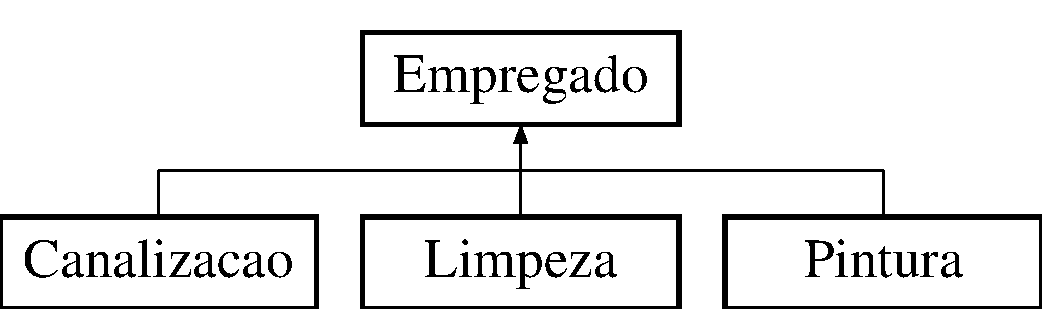
\includegraphics[height=2.000000cm]{class_empregado}
\end{center}
\end{figure}
\subsection*{Public Member Functions}
\begin{DoxyCompactItemize}
\item 
\hyperlink{class_empregado_a41f417a80a0e7e83737c616beede3c7a}{Empregado} (string nome, int bi, string tipo, bool livre)
\begin{DoxyCompactList}\small\item\em Função que cria um empregado. \end{DoxyCompactList}\item 
string \hyperlink{class_empregado_a3b7e1e37085dc3233372303dc5fad063}{get\+Nome} () const 
\begin{DoxyCompactList}\small\item\em Função para obter o nome do empregado. \end{DoxyCompactList}\item 
int \hyperlink{class_empregado_af53f765432478ff43995d6373820a610}{get\+BI} () const 
\begin{DoxyCompactList}\small\item\em Função para obter o número do bilhete de identidade do empregado. \end{DoxyCompactList}\item 
string \hyperlink{class_empregado_a31668a30674046ed45b1543de5948b39}{get\+Tipo} () const 
\begin{DoxyCompactList}\small\item\em Função para obter o tipo de empregado. \end{DoxyCompactList}\item 
bool \hyperlink{class_empregado_a79d9a4467c7c506f26f178fe94f3084d}{get\+Livre} () const 
\begin{DoxyCompactList}\small\item\em Função para verificar se um empregado está livre. \end{DoxyCompactList}\item 
void \hyperlink{class_empregado_a81997099011c547e71bc52c5e69532d9}{set\+Livre} (bool livre)
\begin{DoxyCompactList}\small\item\em Função que altera o estado do empregado para livre ou ocupado. \end{DoxyCompactList}\item 
bool \hyperlink{class_empregado_a853fad9194cfb37648003e7b4acd431c}{operator==} (const \hyperlink{class_empregado}{Empregado} \&empregado)
\begin{DoxyCompactList}\small\item\em Operador para verificar se dois empregados são o mesmo. \end{DoxyCompactList}\end{DoxyCompactItemize}


\subsection{Constructor \& Destructor Documentation}
\index{Empregado@{Empregado}!Empregado@{Empregado}}
\index{Empregado@{Empregado}!Empregado@{Empregado}}
\subsubsection[{Empregado(string nome, int bi, string tipo, bool livre)}]{\setlength{\rightskip}{0pt plus 5cm}Empregado\+::\+Empregado (
\begin{DoxyParamCaption}
\item[{string}]{nome, }
\item[{int}]{bi, }
\item[{string}]{tipo, }
\item[{bool}]{livre}
\end{DoxyParamCaption}
)}\hypertarget{class_empregado_a41f417a80a0e7e83737c616beede3c7a}{}\label{class_empregado_a41f417a80a0e7e83737c616beede3c7a}


Função que cria um empregado. 


\begin{DoxyParams}{Parameters}
{\em nome} & -\/ nome do empregado. \\
\hline
{\em bi} & -\/ número do bilhete de identidade. \\
\hline
{\em livre} & -\/ se for verdadeiro então o empregado está livre, caso contrário está ocupado. \\
\hline
\end{DoxyParams}


\subsection{Member Function Documentation}
\index{Empregado@{Empregado}!get\+BI@{get\+BI}}
\index{get\+BI@{get\+BI}!Empregado@{Empregado}}
\subsubsection[{get\+B\+I() const }]{\setlength{\rightskip}{0pt plus 5cm}int Empregado\+::get\+BI (
\begin{DoxyParamCaption}
{}
\end{DoxyParamCaption}
) const}\hypertarget{class_empregado_af53f765432478ff43995d6373820a610}{}\label{class_empregado_af53f765432478ff43995d6373820a610}


Função para obter o número do bilhete de identidade do empregado. 

\begin{DoxyReturn}{Returns}
Retorna o número do bilhete de identidade do empregado. 
\end{DoxyReturn}
\index{Empregado@{Empregado}!get\+Livre@{get\+Livre}}
\index{get\+Livre@{get\+Livre}!Empregado@{Empregado}}
\subsubsection[{get\+Livre() const }]{\setlength{\rightskip}{0pt plus 5cm}bool Empregado\+::get\+Livre (
\begin{DoxyParamCaption}
{}
\end{DoxyParamCaption}
) const}\hypertarget{class_empregado_a79d9a4467c7c506f26f178fe94f3084d}{}\label{class_empregado_a79d9a4467c7c506f26f178fe94f3084d}


Função para verificar se um empregado está livre. 

\begin{DoxyReturn}{Returns}
Retorna verdadeiro se o empregado está livre e falso caso contrário. 
\end{DoxyReturn}
\index{Empregado@{Empregado}!get\+Nome@{get\+Nome}}
\index{get\+Nome@{get\+Nome}!Empregado@{Empregado}}
\subsubsection[{get\+Nome() const }]{\setlength{\rightskip}{0pt plus 5cm}string Empregado\+::get\+Nome (
\begin{DoxyParamCaption}
{}
\end{DoxyParamCaption}
) const}\hypertarget{class_empregado_a3b7e1e37085dc3233372303dc5fad063}{}\label{class_empregado_a3b7e1e37085dc3233372303dc5fad063}


Função para obter o nome do empregado. 

\begin{DoxyReturn}{Returns}
Retorna o nome do empregado. 
\end{DoxyReturn}
\index{Empregado@{Empregado}!get\+Tipo@{get\+Tipo}}
\index{get\+Tipo@{get\+Tipo}!Empregado@{Empregado}}
\subsubsection[{get\+Tipo() const }]{\setlength{\rightskip}{0pt plus 5cm}string Empregado\+::get\+Tipo (
\begin{DoxyParamCaption}
{}
\end{DoxyParamCaption}
) const}\hypertarget{class_empregado_a31668a30674046ed45b1543de5948b39}{}\label{class_empregado_a31668a30674046ed45b1543de5948b39}


Função para obter o tipo de empregado. 

\begin{DoxyReturn}{Returns}
Retorna o tipo de empregado. 
\end{DoxyReturn}
\index{Empregado@{Empregado}!operator==@{operator==}}
\index{operator==@{operator==}!Empregado@{Empregado}}
\subsubsection[{operator==(const Empregado \&empregado)}]{\setlength{\rightskip}{0pt plus 5cm}bool Empregado\+::operator== (
\begin{DoxyParamCaption}
\item[{const {\bf Empregado} \&}]{empregado}
\end{DoxyParamCaption}
)}\hypertarget{class_empregado_a853fad9194cfb37648003e7b4acd431c}{}\label{class_empregado_a853fad9194cfb37648003e7b4acd431c}


Operador para verificar se dois empregados são o mesmo. 


\begin{DoxyParams}{Parameters}
{\em empregado} & -\/ empregado externo com a qual vai ser comparado o empregado. \\
\hline
\end{DoxyParams}
\begin{DoxyReturn}{Returns}
Retorna verdade caso os empregados sejam o mesmo e falso caso contrário. 
\end{DoxyReturn}
\index{Empregado@{Empregado}!set\+Livre@{set\+Livre}}
\index{set\+Livre@{set\+Livre}!Empregado@{Empregado}}
\subsubsection[{set\+Livre(bool livre)}]{\setlength{\rightskip}{0pt plus 5cm}void Empregado\+::set\+Livre (
\begin{DoxyParamCaption}
\item[{bool}]{livre}
\end{DoxyParamCaption}
)}\hypertarget{class_empregado_a81997099011c547e71bc52c5e69532d9}{}\label{class_empregado_a81997099011c547e71bc52c5e69532d9}


Função que altera o estado do empregado para livre ou ocupado. 


\begin{DoxyParams}{Parameters}
{\em livre} & -\/ valor que indica se se quer alterar o empregado para livre ou para ocupado. \\
\hline
\end{DoxyParams}


The documentation for this class was generated from the following files\+:\begin{DoxyCompactItemize}
\item 
Empregado.\+h\item 
Empregado.\+cpp\end{DoxyCompactItemize}

\hypertarget{class_empregado_existente}{}\section{Empregado\+Existente Class Reference}
\label{class_empregado_existente}\index{Empregado\+Existente@{Empregado\+Existente}}
\subsection*{Public Member Functions}
\begin{DoxyCompactItemize}
\item 
\hyperlink{class_empregado_existente_a70f63c83220ff5401b43a019146d53c5}{Empregado\+Existente} (int num\+\_\+bi)
\begin{DoxyCompactList}\small\item\em Cria exceção quando se tenta adicionar um empregado que já existe. \end{DoxyCompactList}\item 
int \hyperlink{class_empregado_existente_aac09f5b67a54a429bb263d7db3dfb43f}{get\+BI} () const 
\begin{DoxyCompactList}\small\item\em Função para obter o número do bilhete de identidade do empregado. \end{DoxyCompactList}\end{DoxyCompactItemize}


\subsection{Constructor \& Destructor Documentation}
\index{Empregado\+Existente@{Empregado\+Existente}!Empregado\+Existente@{Empregado\+Existente}}
\index{Empregado\+Existente@{Empregado\+Existente}!Empregado\+Existente@{Empregado\+Existente}}
\subsubsection[{Empregado\+Existente(int num\+\_\+bi)}]{\setlength{\rightskip}{0pt plus 5cm}Empregado\+Existente\+::\+Empregado\+Existente (
\begin{DoxyParamCaption}
\item[{int}]{num\+\_\+bi}
\end{DoxyParamCaption}
)}\hypertarget{class_empregado_existente_a70f63c83220ff5401b43a019146d53c5}{}\label{class_empregado_existente_a70f63c83220ff5401b43a019146d53c5}


Cria exceção quando se tenta adicionar um empregado que já existe. 


\begin{DoxyParams}{Parameters}
{\em num\+\_\+bi} & -\/ Número do bilhete de identidade do empregado. \\
\hline
\end{DoxyParams}


\subsection{Member Function Documentation}
\index{Empregado\+Existente@{Empregado\+Existente}!get\+BI@{get\+BI}}
\index{get\+BI@{get\+BI}!Empregado\+Existente@{Empregado\+Existente}}
\subsubsection[{get\+B\+I() const }]{\setlength{\rightskip}{0pt plus 5cm}int Empregado\+Existente\+::get\+BI (
\begin{DoxyParamCaption}
{}
\end{DoxyParamCaption}
) const}\hypertarget{class_empregado_existente_aac09f5b67a54a429bb263d7db3dfb43f}{}\label{class_empregado_existente_aac09f5b67a54a429bb263d7db3dfb43f}


Função para obter o número do bilhete de identidade do empregado. 

\begin{DoxyReturn}{Returns}
Retorna o número do bilhete de identidade do empregado. 
\end{DoxyReturn}


The documentation for this class was generated from the following files\+:\begin{DoxyCompactItemize}
\item 
excecoes.\+h\item 
excecoes.\+cpp\end{DoxyCompactItemize}

\hypertarget{class_habitacao}{}\section{Habitacao Class Reference}
\label{class_habitacao}\index{Habitacao@{Habitacao}}
Inheritance diagram for Habitacao\+:\begin{figure}[H]
\begin{center}
\leavevmode
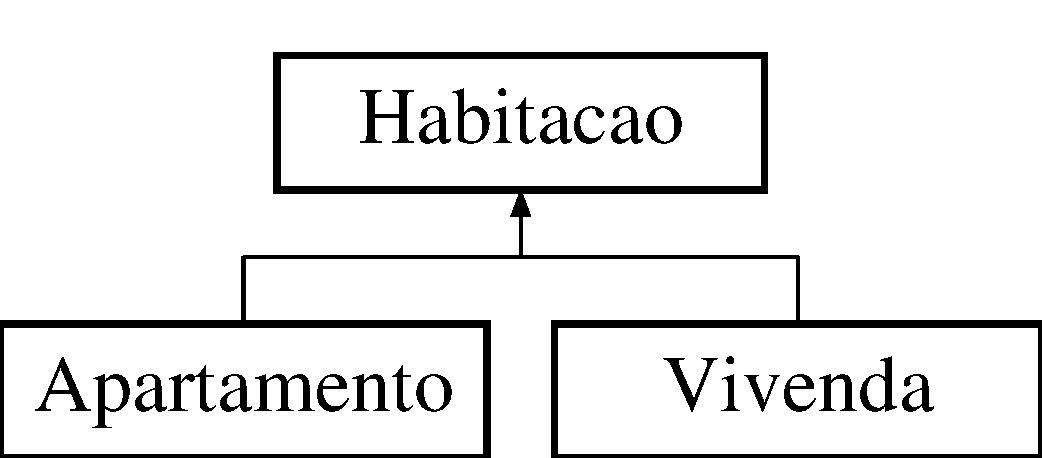
\includegraphics[height=2.000000cm]{class_habitacao}
\end{center}
\end{figure}
\subsection*{Public Member Functions}
\begin{DoxyCompactItemize}
\item 
\hyperlink{class_habitacao_a3b5e5edb0ca3b52025ef46a796fcf18d}{Habitacao} (string morada, int area\+Habitacao)
\begin{DoxyCompactList}\small\item\em Função que cria uma habitação. \end{DoxyCompactList}\item 
virtual float \hyperlink{class_habitacao_a479d2307661c87b05242b86ba849fb6e}{mensalidade} () const 
\begin{DoxyCompactList}\small\item\em Função que calcula o valor da base mensal de condomínio. \end{DoxyCompactList}\item 
string \hyperlink{class_habitacao_a17ef78eef7746f92bd2814893bfafbab}{get\+Morada} () const 
\begin{DoxyCompactList}\small\item\em Função para obter a morada da habitação. \end{DoxyCompactList}\item 
int \hyperlink{class_habitacao_a8b8dc61b41f3bda37f3e517fe63f877a}{get\+Area\+Habitacao} () const 
\begin{DoxyCompactList}\small\item\em Função para obter a area habitacional. \end{DoxyCompactList}\item 
bool \hyperlink{class_habitacao_acd290b8d83f41d4667867d5dc353166e}{operator==} (const \hyperlink{class_habitacao}{Habitacao} \&hab)
\begin{DoxyCompactList}\small\item\em Operador para verificar se duas habitações são a mesma. \end{DoxyCompactList}\item 
void \hyperlink{class_habitacao_a2a8c7343f36b0d9415aef14b09bca511}{adiciona\+Servico} (\hyperlink{class_empregado}{Empregado} $\ast$servico)
\begin{DoxyCompactList}\small\item\em Adiciona um serviço ao histórico de serviços. \end{DoxyCompactList}\end{DoxyCompactItemize}


\subsection{Constructor \& Destructor Documentation}
\index{Habitacao@{Habitacao}!Habitacao@{Habitacao}}
\index{Habitacao@{Habitacao}!Habitacao@{Habitacao}}
\subsubsection[{Habitacao(string morada, int area\+Habitacao)}]{\setlength{\rightskip}{0pt plus 5cm}Habitacao\+::\+Habitacao (
\begin{DoxyParamCaption}
\item[{string}]{morada, }
\item[{int}]{area\+Habitacao}
\end{DoxyParamCaption}
)}\hypertarget{class_habitacao_a3b5e5edb0ca3b52025ef46a796fcf18d}{}\label{class_habitacao_a3b5e5edb0ca3b52025ef46a796fcf18d}


Função que cria uma habitação. 


\begin{DoxyParams}{Parameters}
{\em morada} & -\/ localização geográfica da habitação. \\
\hline
{\em area\+Habitacao} & -\/ area habitacional. \\
\hline
\end{DoxyParams}


\subsection{Member Function Documentation}
\index{Habitacao@{Habitacao}!adiciona\+Servico@{adiciona\+Servico}}
\index{adiciona\+Servico@{adiciona\+Servico}!Habitacao@{Habitacao}}
\subsubsection[{adiciona\+Servico(\+Empregado $\ast$servico)}]{\setlength{\rightskip}{0pt plus 5cm}void Habitacao\+::adiciona\+Servico (
\begin{DoxyParamCaption}
\item[{{\bf Empregado} $\ast$}]{servico}
\end{DoxyParamCaption}
)}\hypertarget{class_habitacao_a2a8c7343f36b0d9415aef14b09bca511}{}\label{class_habitacao_a2a8c7343f36b0d9415aef14b09bca511}


Adiciona um serviço ao histórico de serviços. 


\begin{DoxyParams}{Parameters}
{\em servico} & -\/ servico que foi requisitado. \\
\hline
\end{DoxyParams}
\index{Habitacao@{Habitacao}!get\+Area\+Habitacao@{get\+Area\+Habitacao}}
\index{get\+Area\+Habitacao@{get\+Area\+Habitacao}!Habitacao@{Habitacao}}
\subsubsection[{get\+Area\+Habitacao() const }]{\setlength{\rightskip}{0pt plus 5cm}int Habitacao\+::get\+Area\+Habitacao (
\begin{DoxyParamCaption}
{}
\end{DoxyParamCaption}
) const}\hypertarget{class_habitacao_a8b8dc61b41f3bda37f3e517fe63f877a}{}\label{class_habitacao_a8b8dc61b41f3bda37f3e517fe63f877a}


Função para obter a area habitacional. 

\begin{DoxyReturn}{Returns}
Retorna a area habitacional. 
\end{DoxyReturn}
\index{Habitacao@{Habitacao}!get\+Morada@{get\+Morada}}
\index{get\+Morada@{get\+Morada}!Habitacao@{Habitacao}}
\subsubsection[{get\+Morada() const }]{\setlength{\rightskip}{0pt plus 5cm}string Habitacao\+::get\+Morada (
\begin{DoxyParamCaption}
{}
\end{DoxyParamCaption}
) const}\hypertarget{class_habitacao_a17ef78eef7746f92bd2814893bfafbab}{}\label{class_habitacao_a17ef78eef7746f92bd2814893bfafbab}


Função para obter a morada da habitação. 

\begin{DoxyReturn}{Returns}
Retorna a morada da habitação. 
\end{DoxyReturn}
\index{Habitacao@{Habitacao}!mensalidade@{mensalidade}}
\index{mensalidade@{mensalidade}!Habitacao@{Habitacao}}
\subsubsection[{mensalidade() const }]{\setlength{\rightskip}{0pt plus 5cm}float Habitacao\+::mensalidade (
\begin{DoxyParamCaption}
{}
\end{DoxyParamCaption}
) const\hspace{0.3cm}{\ttfamily [virtual]}}\hypertarget{class_habitacao_a479d2307661c87b05242b86ba849fb6e}{}\label{class_habitacao_a479d2307661c87b05242b86ba849fb6e}


Função que calcula o valor da base mensal de condomínio. 

\begin{DoxyReturn}{Returns}
Retorna o valor da base mensal de condomínio. 
\end{DoxyReturn}


Reimplemented in \hyperlink{class_vivenda_ad542e2b2f31da8c24b706211efc880d8}{Vivenda}, and \hyperlink{class_apartamento_a3626df5dabd6871c5f9fce39e8c70249}{Apartamento}.

\index{Habitacao@{Habitacao}!operator==@{operator==}}
\index{operator==@{operator==}!Habitacao@{Habitacao}}
\subsubsection[{operator==(const Habitacao \&hab)}]{\setlength{\rightskip}{0pt plus 5cm}bool Habitacao\+::operator== (
\begin{DoxyParamCaption}
\item[{const {\bf Habitacao} \&}]{hab}
\end{DoxyParamCaption}
)}\hypertarget{class_habitacao_acd290b8d83f41d4667867d5dc353166e}{}\label{class_habitacao_acd290b8d83f41d4667867d5dc353166e}


Operador para verificar se duas habitações são a mesma. 


\begin{DoxyParams}{Parameters}
{\em hab} & -\/ habitação externa com a qual vai ser comparada a habitação. \\
\hline
\end{DoxyParams}
\begin{DoxyReturn}{Returns}
Retorna verdade caso as habitações sejam a mesma e falso caso contrário. 
\end{DoxyReturn}


The documentation for this class was generated from the following files\+:\begin{DoxyCompactItemize}
\item 
Habitacao.\+h\item 
Habitacao.\+cpp\end{DoxyCompactItemize}

\hypertarget{class_limite_maximo_empregados}{}\section{Limite\+Maximo\+Empregados Class Reference}
\label{class_limite_maximo_empregados}\index{Limite\+Maximo\+Empregados@{Limite\+Maximo\+Empregados}}
\subsection*{Public Member Functions}
\begin{DoxyCompactItemize}
\item 
\hyperlink{class_limite_maximo_empregados_a5b3f5383d238e8b7791c05d3b09bc987}{Limite\+Maximo\+Empregados} (string t)
\begin{DoxyCompactList}\small\item\em Cria exceção para quando se tenta adicionar um empregado de um tipo que já atingiu o limite máximo definido pela empresa de serviços. \end{DoxyCompactList}\item 
string \hyperlink{class_limite_maximo_empregados_ad7fe69080cc2cafa0ad4fd6d1ffdcb84}{get\+Tipo} () const 
\begin{DoxyCompactList}\small\item\em Função para obter o tipo de empregado. \end{DoxyCompactList}\end{DoxyCompactItemize}


\subsection{Constructor \& Destructor Documentation}
\index{Limite\+Maximo\+Empregados@{Limite\+Maximo\+Empregados}!Limite\+Maximo\+Empregados@{Limite\+Maximo\+Empregados}}
\index{Limite\+Maximo\+Empregados@{Limite\+Maximo\+Empregados}!Limite\+Maximo\+Empregados@{Limite\+Maximo\+Empregados}}
\subsubsection[{Limite\+Maximo\+Empregados(string t)}]{\setlength{\rightskip}{0pt plus 5cm}Limite\+Maximo\+Empregados\+::\+Limite\+Maximo\+Empregados (
\begin{DoxyParamCaption}
\item[{string}]{t}
\end{DoxyParamCaption}
)}\hypertarget{class_limite_maximo_empregados_a5b3f5383d238e8b7791c05d3b09bc987}{}\label{class_limite_maximo_empregados_a5b3f5383d238e8b7791c05d3b09bc987}


Cria exceção para quando se tenta adicionar um empregado de um tipo que já atingiu o limite máximo definido pela empresa de serviços. 


\begin{DoxyParams}{Parameters}
{\em t} & -\/ tipo de empregado. \\
\hline
\end{DoxyParams}


\subsection{Member Function Documentation}
\index{Limite\+Maximo\+Empregados@{Limite\+Maximo\+Empregados}!get\+Tipo@{get\+Tipo}}
\index{get\+Tipo@{get\+Tipo}!Limite\+Maximo\+Empregados@{Limite\+Maximo\+Empregados}}
\subsubsection[{get\+Tipo() const }]{\setlength{\rightskip}{0pt plus 5cm}string Limite\+Maximo\+Empregados\+::get\+Tipo (
\begin{DoxyParamCaption}
{}
\end{DoxyParamCaption}
) const}\hypertarget{class_limite_maximo_empregados_ad7fe69080cc2cafa0ad4fd6d1ffdcb84}{}\label{class_limite_maximo_empregados_ad7fe69080cc2cafa0ad4fd6d1ffdcb84}


Função para obter o tipo de empregado. 

\begin{DoxyReturn}{Returns}
Retorna o tipo de empregado. 
\end{DoxyReturn}


The documentation for this class was generated from the following files\+:\begin{DoxyCompactItemize}
\item 
excecoes.\+h\item 
excecoes.\+cpp\end{DoxyCompactItemize}

\hypertarget{class_limpeza}{}\section{Limpeza Class Reference}
\label{class_limpeza}\index{Limpeza@{Limpeza}}
Inheritance diagram for Limpeza\+:\begin{figure}[H]
\begin{center}
\leavevmode
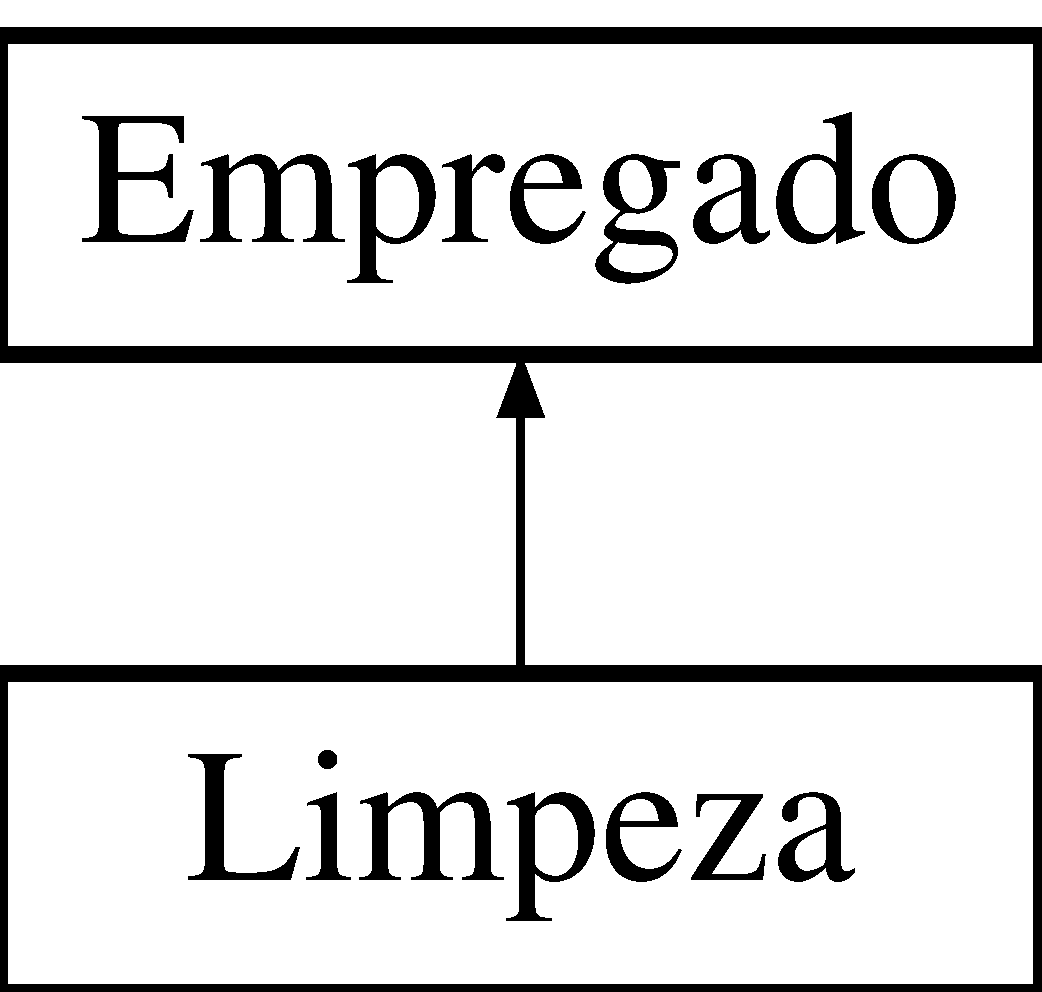
\includegraphics[height=2.000000cm]{class_limpeza}
\end{center}
\end{figure}
\subsection*{Public Member Functions}
\begin{DoxyCompactItemize}
\item 
\hyperlink{class_limpeza_ae247b833f8e8bc16d70164bbfbf2bd67}{Limpeza} (string nome, int bi, string tipo, bool livre)
\begin{DoxyCompactList}\small\item\em Função que cria um empregado de limpeza. \end{DoxyCompactList}\end{DoxyCompactItemize}


\subsection{Constructor \& Destructor Documentation}
\index{Limpeza@{Limpeza}!Limpeza@{Limpeza}}
\index{Limpeza@{Limpeza}!Limpeza@{Limpeza}}
\subsubsection[{Limpeza(string nome, int bi, string tipo, bool livre)}]{\setlength{\rightskip}{0pt plus 5cm}Limpeza\+::\+Limpeza (
\begin{DoxyParamCaption}
\item[{string}]{nome, }
\item[{int}]{bi, }
\item[{string}]{tipo, }
\item[{bool}]{livre}
\end{DoxyParamCaption}
)}\hypertarget{class_limpeza_ae247b833f8e8bc16d70164bbfbf2bd67}{}\label{class_limpeza_ae247b833f8e8bc16d70164bbfbf2bd67}


Função que cria um empregado de limpeza. 


\begin{DoxyParams}{Parameters}
{\em nome} & -\/ nome do empregado. \\
\hline
{\em bi} & -\/ número do bilhete de identidade. \\
\hline
{\em tipo} & -\/ o tipo deve ser \char`\"{}limpeza\char`\"{}, caso contrário é lançada uma exceção. \\
\hline
{\em livre} & -\/ se for verdadeiro então o empregado está livre, caso contrário está ocupado. \\
\hline
\end{DoxyParams}


The documentation for this class was generated from the following files\+:\begin{DoxyCompactItemize}
\item 
Limpeza.\+h\item 
Limpeza.\+cpp\end{DoxyCompactItemize}

\hypertarget{class_pintura}{}\section{Pintura Class Reference}
\label{class_pintura}\index{Pintura@{Pintura}}
Inheritance diagram for Pintura\+:\begin{figure}[H]
\begin{center}
\leavevmode
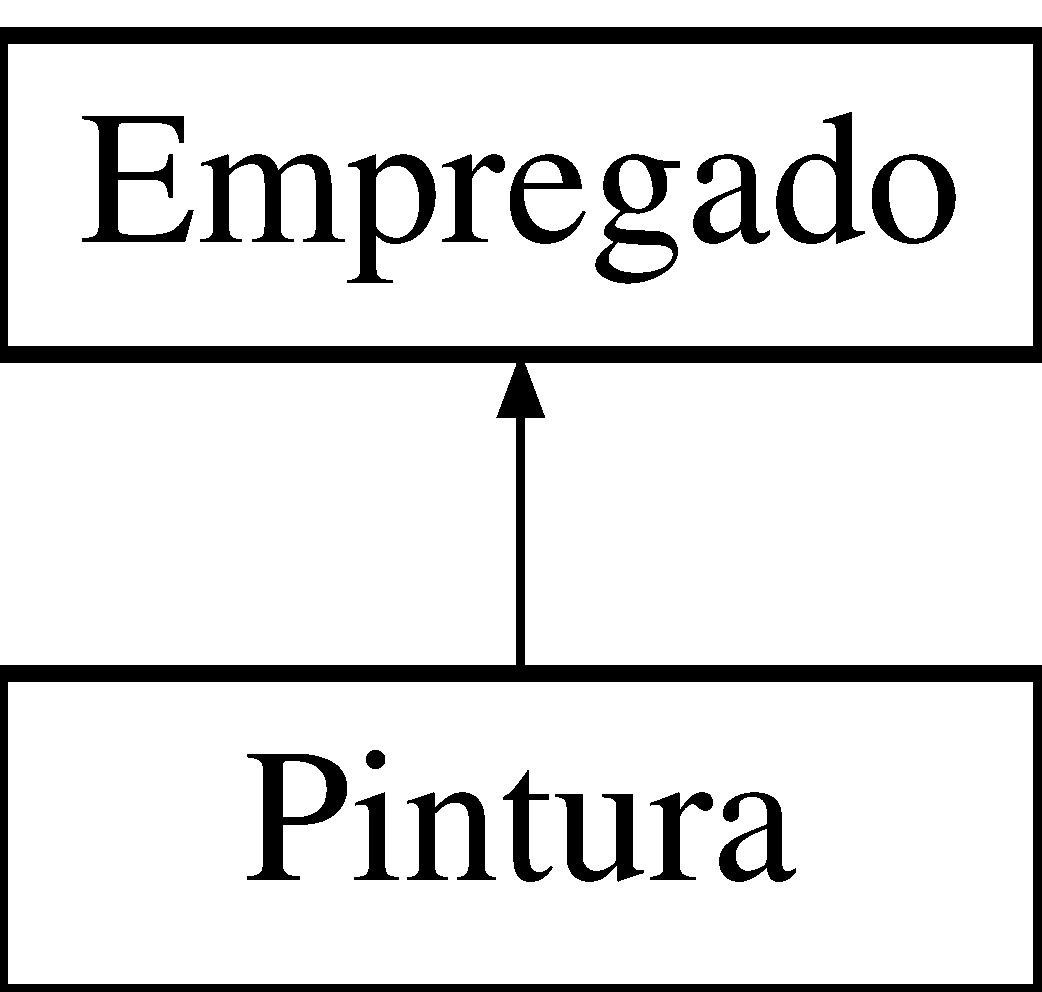
\includegraphics[height=2.000000cm]{class_pintura}
\end{center}
\end{figure}
\subsection*{Public Member Functions}
\begin{DoxyCompactItemize}
\item 
\hyperlink{class_pintura_abfd65a4c901ffe3a2d9f0a4da8e9a98d}{Pintura} (string nome, int bi, int numero\+Telemovel, string email, string tipo, bool livre)
\begin{DoxyCompactList}\small\item\em Função que cria um empregado de pintura. \end{DoxyCompactList}\end{DoxyCompactItemize}


\subsection{Constructor \& Destructor Documentation}
\index{Pintura@{Pintura}!Pintura@{Pintura}}
\index{Pintura@{Pintura}!Pintura@{Pintura}}
\subsubsection[{Pintura(string nome, int bi, int numero\+Telemovel, string email, string tipo, bool livre)}]{\setlength{\rightskip}{0pt plus 5cm}Pintura\+::\+Pintura (
\begin{DoxyParamCaption}
\item[{string}]{nome, }
\item[{int}]{bi, }
\item[{int}]{numero\+Telemovel, }
\item[{string}]{email, }
\item[{string}]{tipo, }
\item[{bool}]{livre}
\end{DoxyParamCaption}
)}\hypertarget{class_pintura_abfd65a4c901ffe3a2d9f0a4da8e9a98d}{}\label{class_pintura_abfd65a4c901ffe3a2d9f0a4da8e9a98d}


Função que cria um empregado de pintura. 


\begin{DoxyParams}{Parameters}
{\em nome} & -\/ nome do empregado. \\
\hline
{\em bi} & -\/ número do bilhete de identidade. \\
\hline
{\em numero\+Telemovel} & -\/ número de telemóvel do empregado. \\
\hline
{\em email} & -\/ email do empregado. \\
\hline
{\em tipo} & -\/ o tipo deve ser \char`\"{}pintura\char`\"{}, caso contrário é lançada uma exceção. \\
\hline
{\em livre} & -\/ se for verdadeiro então o empregado está livre, caso contrário está ocupado. \\
\hline
\end{DoxyParams}


The documentation for this class was generated from the following files\+:\begin{DoxyCompactItemize}
\item 
Pintura.\+h\item 
Pintura.\+cpp\end{DoxyCompactItemize}

\hypertarget{class_servico}{}\section{Servico Class Reference}
\label{class_servico}\index{Servico@{Servico}}
\subsection*{Public Member Functions}
\begin{DoxyCompactItemize}
\item 
\hyperlink{class_servico_a920dbd3231fa6ca3ba9e118764bb7d4b}{Servico} (vector$<$ \hyperlink{class_empregado}{Empregado} $\ast$ $>$ empregados, int max\+Emp\+Limpeza, int max\+Emp\+Canalizacao, int max\+Emp\+Pintura)
\begin{DoxyCompactList}\small\item\em Função que cria uma empresa de serviços. \end{DoxyCompactList}\item 
int \hyperlink{class_servico_a590ca90b6563c337eeb55b08255a4894}{num\+Emp\+Limpeza} () const 
\begin{DoxyCompactList}\small\item\em Função para obter o número de empregados de limpeza existentes. \end{DoxyCompactList}\item 
int \hyperlink{class_servico_a09dedacf7c261a12e86e263510748c74}{num\+Emp\+Canalizacao} () const 
\begin{DoxyCompactList}\small\item\em Função para obter o número de canalizadores existentes. \end{DoxyCompactList}\item 
int \hyperlink{class_servico_a9e2a6c88d5e6aa250fe4472cd2cec3bf}{num\+Emp\+Pintura} () const 
\begin{DoxyCompactList}\small\item\em Função para obter o número de pintores existentes. \end{DoxyCompactList}\item 
int \hyperlink{class_servico_a6cd98c383025f6a00a4314caab86a016}{num\+Emp\+Limpeza\+Livres} () const 
\begin{DoxyCompactList}\small\item\em Função para obter o número de empregados de limpeza livres. \end{DoxyCompactList}\item 
int \hyperlink{class_servico_a459265d6c8a9a6e5e4c33e8aada812bb}{num\+Emp\+Canalizacao\+Livres} () const 
\begin{DoxyCompactList}\small\item\em Função para obter o número de canalizadores livres. \end{DoxyCompactList}\item 
int \hyperlink{class_servico_a83583e1dca00f51715e03a1f33818494}{num\+Emp\+Pintura\+Livres} () const 
\begin{DoxyCompactList}\small\item\em Função para obter o número de pintores livres. \end{DoxyCompactList}\item 
int \hyperlink{class_servico_a6e3eb546bad5975cf8e678ae4e6f6ea3}{adiciona\+Empregado} (\hyperlink{class_empregado}{Empregado} $\ast$empregado)
\begin{DoxyCompactList}\small\item\em Adiciona um empregado aos empregados da empresa de serviços. \end{DoxyCompactList}\item 
int \hyperlink{class_servico_af2d0e60b4f9b4c1a3e9c545d00a87659}{remove\+Empregado} (\hyperlink{class_empregado}{Empregado} $\ast$empregado)
\begin{DoxyCompactList}\small\item\em Remove um empregado dos empregados da empresa. \end{DoxyCompactList}\item 
int \hyperlink{class_servico_a1a9fbbe6413835ba366355cc4131c413}{get\+Servicos\+Disponiveis} () const 
\begin{DoxyCompactList}\small\item\em Função para obter o número de empregados que estão livres na empresa de serviços. \end{DoxyCompactList}\item 
vector$<$ \hyperlink{class_empregado}{Empregado} $\ast$ $>$ \hyperlink{class_servico_a9d7003d0cc174b05ee16b329d4c96b44}{get\+Empregados} () const 
\begin{DoxyCompactList}\small\item\em Função para obter os empregados da empresa de serviços. \end{DoxyCompactList}\item 
int \hyperlink{class_servico_a61f4dc0bff250f3be3c23b495c2b0e91}{dec\+Servicos\+Disponiveis} ()
\begin{DoxyCompactList}\small\item\em Função decrementa o número de servicos disponiveis. \end{DoxyCompactList}\item 
int \hyperlink{class_servico_a099b6ca2af6f7d577d1fe6b36349975c}{inc\+Servicos\+Disponiveis} ()
\begin{DoxyCompactList}\small\item\em Função incrementa o número de servicos disponiveis. \end{DoxyCompactList}\item 
int \hyperlink{class_servico_a019fcbffefddc52608ee3e34a8479e85}{get\+Num\+Max\+Limpeza} () const 
\begin{DoxyCompactList}\small\item\em Função para obter o número máximo de empregados de limpeza permitidos. \end{DoxyCompactList}\item 
int \hyperlink{class_servico_a74c8980bc7ca92ce7cc6f9e41d73ca38}{get\+Num\+Max\+Canalizacao} () const 
\begin{DoxyCompactList}\small\item\em Função para obter o número máximo de canalizadores permitidos. \end{DoxyCompactList}\item 
int \hyperlink{class_servico_a34c593b378ec48353f86e807644fa97e}{get\+Num\+Max\+Pintura} () const 
\begin{DoxyCompactList}\small\item\em Função para obter o número máximo de pintores permitidos. \end{DoxyCompactList}\end{DoxyCompactItemize}


\subsection{Constructor \& Destructor Documentation}
\index{Servico@{Servico}!Servico@{Servico}}
\index{Servico@{Servico}!Servico@{Servico}}
\subsubsection[{Servico(vector$<$ Empregado $\ast$ $>$ empregados, int max\+Emp\+Limpeza, int max\+Emp\+Canalizacao, int max\+Emp\+Pintura)}]{\setlength{\rightskip}{0pt plus 5cm}Servico\+::\+Servico (
\begin{DoxyParamCaption}
\item[{vector$<$ {\bf Empregado} $\ast$ $>$}]{empregados, }
\item[{int}]{max\+Emp\+Limpeza, }
\item[{int}]{max\+Emp\+Canalizacao, }
\item[{int}]{max\+Emp\+Pintura}
\end{DoxyParamCaption}
)}\hypertarget{class_servico_a920dbd3231fa6ca3ba9e118764bb7d4b}{}\label{class_servico_a920dbd3231fa6ca3ba9e118764bb7d4b}


Função que cria uma empresa de serviços. 


\begin{DoxyParams}{Parameters}
{\em empregados} & -\/ empregados da empresa. \\
\hline
{\em max\+Emp\+Limpeza} & -\/ número máximo de empregados de limpeza permitidos nesta empresa. \\
\hline
{\em max\+Emp\+Canalizacao} & -\/ número máximo de canalizadores permitidos nesta empresa. \\
\hline
{\em max\+Emp\+Pintura} & -\/ número máximo de pintores permitidos nesta empresa. \\
\hline
\end{DoxyParams}


\subsection{Member Function Documentation}
\index{Servico@{Servico}!adiciona\+Empregado@{adiciona\+Empregado}}
\index{adiciona\+Empregado@{adiciona\+Empregado}!Servico@{Servico}}
\subsubsection[{adiciona\+Empregado(\+Empregado $\ast$empregado)}]{\setlength{\rightskip}{0pt plus 5cm}int Servico\+::adiciona\+Empregado (
\begin{DoxyParamCaption}
\item[{{\bf Empregado} $\ast$}]{empregado}
\end{DoxyParamCaption}
)}\hypertarget{class_servico_a6e3eb546bad5975cf8e678ae4e6f6ea3}{}\label{class_servico_a6e3eb546bad5975cf8e678ae4e6f6ea3}


Adiciona um empregado aos empregados da empresa de serviços. 


\begin{DoxyParams}{Parameters}
{\em empregado} & -\/ empregado que se quer adicionar aos empregados da empresa de serviços. \\
\hline
\end{DoxyParams}
\begin{DoxyReturn}{Returns}
Retorna 0 em caso de sucesso. 
\end{DoxyReturn}
\index{Servico@{Servico}!dec\+Servicos\+Disponiveis@{dec\+Servicos\+Disponiveis}}
\index{dec\+Servicos\+Disponiveis@{dec\+Servicos\+Disponiveis}!Servico@{Servico}}
\subsubsection[{dec\+Servicos\+Disponiveis()}]{\setlength{\rightskip}{0pt plus 5cm}int Servico\+::dec\+Servicos\+Disponiveis (
\begin{DoxyParamCaption}
{}
\end{DoxyParamCaption}
)}\hypertarget{class_servico_a61f4dc0bff250f3be3c23b495c2b0e91}{}\label{class_servico_a61f4dc0bff250f3be3c23b495c2b0e91}


Função decrementa o número de servicos disponiveis. 

\begin{DoxyReturn}{Returns}
Retorna 0 em caso de sucesso e -\/1 caso contrário. 
\end{DoxyReturn}
\index{Servico@{Servico}!get\+Empregados@{get\+Empregados}}
\index{get\+Empregados@{get\+Empregados}!Servico@{Servico}}
\subsubsection[{get\+Empregados() const }]{\setlength{\rightskip}{0pt plus 5cm}vector$<$ {\bf Empregado} $\ast$ $>$ Servico\+::get\+Empregados (
\begin{DoxyParamCaption}
{}
\end{DoxyParamCaption}
) const}\hypertarget{class_servico_a9d7003d0cc174b05ee16b329d4c96b44}{}\label{class_servico_a9d7003d0cc174b05ee16b329d4c96b44}


Função para obter os empregados da empresa de serviços. 

\begin{DoxyReturn}{Returns}
Retorna os empregados da empresa de serviços. 
\end{DoxyReturn}
\index{Servico@{Servico}!get\+Num\+Max\+Canalizacao@{get\+Num\+Max\+Canalizacao}}
\index{get\+Num\+Max\+Canalizacao@{get\+Num\+Max\+Canalizacao}!Servico@{Servico}}
\subsubsection[{get\+Num\+Max\+Canalizacao() const }]{\setlength{\rightskip}{0pt plus 5cm}int Servico\+::get\+Num\+Max\+Canalizacao (
\begin{DoxyParamCaption}
{}
\end{DoxyParamCaption}
) const}\hypertarget{class_servico_a74c8980bc7ca92ce7cc6f9e41d73ca38}{}\label{class_servico_a74c8980bc7ca92ce7cc6f9e41d73ca38}


Função para obter o número máximo de canalizadores permitidos. 

\begin{DoxyReturn}{Returns}
Retorna o número máximo de canalizadores permitidos. 
\end{DoxyReturn}
\index{Servico@{Servico}!get\+Num\+Max\+Limpeza@{get\+Num\+Max\+Limpeza}}
\index{get\+Num\+Max\+Limpeza@{get\+Num\+Max\+Limpeza}!Servico@{Servico}}
\subsubsection[{get\+Num\+Max\+Limpeza() const }]{\setlength{\rightskip}{0pt plus 5cm}int Servico\+::get\+Num\+Max\+Limpeza (
\begin{DoxyParamCaption}
{}
\end{DoxyParamCaption}
) const}\hypertarget{class_servico_a019fcbffefddc52608ee3e34a8479e85}{}\label{class_servico_a019fcbffefddc52608ee3e34a8479e85}


Função para obter o número máximo de empregados de limpeza permitidos. 

\begin{DoxyReturn}{Returns}
Retorna o número máximo de empregados de limpeza permitidos. 
\end{DoxyReturn}
\index{Servico@{Servico}!get\+Num\+Max\+Pintura@{get\+Num\+Max\+Pintura}}
\index{get\+Num\+Max\+Pintura@{get\+Num\+Max\+Pintura}!Servico@{Servico}}
\subsubsection[{get\+Num\+Max\+Pintura() const }]{\setlength{\rightskip}{0pt plus 5cm}int Servico\+::get\+Num\+Max\+Pintura (
\begin{DoxyParamCaption}
{}
\end{DoxyParamCaption}
) const}\hypertarget{class_servico_a34c593b378ec48353f86e807644fa97e}{}\label{class_servico_a34c593b378ec48353f86e807644fa97e}


Função para obter o número máximo de pintores permitidos. 

\begin{DoxyReturn}{Returns}
Retorna o número máximo de pintores permitidos. 
\end{DoxyReturn}
\index{Servico@{Servico}!get\+Servicos\+Disponiveis@{get\+Servicos\+Disponiveis}}
\index{get\+Servicos\+Disponiveis@{get\+Servicos\+Disponiveis}!Servico@{Servico}}
\subsubsection[{get\+Servicos\+Disponiveis() const }]{\setlength{\rightskip}{0pt plus 5cm}int Servico\+::get\+Servicos\+Disponiveis (
\begin{DoxyParamCaption}
{}
\end{DoxyParamCaption}
) const}\hypertarget{class_servico_a1a9fbbe6413835ba366355cc4131c413}{}\label{class_servico_a1a9fbbe6413835ba366355cc4131c413}


Função para obter o número de empregados que estão livres na empresa de serviços. 

\begin{DoxyReturn}{Returns}
Retorna o número de empregados que estão livres na empresa de serviços. 
\end{DoxyReturn}
\index{Servico@{Servico}!inc\+Servicos\+Disponiveis@{inc\+Servicos\+Disponiveis}}
\index{inc\+Servicos\+Disponiveis@{inc\+Servicos\+Disponiveis}!Servico@{Servico}}
\subsubsection[{inc\+Servicos\+Disponiveis()}]{\setlength{\rightskip}{0pt plus 5cm}int Servico\+::inc\+Servicos\+Disponiveis (
\begin{DoxyParamCaption}
{}
\end{DoxyParamCaption}
)}\hypertarget{class_servico_a099b6ca2af6f7d577d1fe6b36349975c}{}\label{class_servico_a099b6ca2af6f7d577d1fe6b36349975c}


Função incrementa o número de servicos disponiveis. 

\begin{DoxyReturn}{Returns}
Retorna 0 em caso de sucesso e -\/1 caso contrário. 
\end{DoxyReturn}
\index{Servico@{Servico}!num\+Emp\+Canalizacao@{num\+Emp\+Canalizacao}}
\index{num\+Emp\+Canalizacao@{num\+Emp\+Canalizacao}!Servico@{Servico}}
\subsubsection[{num\+Emp\+Canalizacao() const }]{\setlength{\rightskip}{0pt plus 5cm}int Servico\+::num\+Emp\+Canalizacao (
\begin{DoxyParamCaption}
{}
\end{DoxyParamCaption}
) const}\hypertarget{class_servico_a09dedacf7c261a12e86e263510748c74}{}\label{class_servico_a09dedacf7c261a12e86e263510748c74}


Função para obter o número de canalizadores existentes. 

\begin{DoxyReturn}{Returns}
Retorna o número de canalizadores existentes. 
\end{DoxyReturn}
\index{Servico@{Servico}!num\+Emp\+Canalizacao\+Livres@{num\+Emp\+Canalizacao\+Livres}}
\index{num\+Emp\+Canalizacao\+Livres@{num\+Emp\+Canalizacao\+Livres}!Servico@{Servico}}
\subsubsection[{num\+Emp\+Canalizacao\+Livres() const }]{\setlength{\rightskip}{0pt plus 5cm}int Servico\+::num\+Emp\+Canalizacao\+Livres (
\begin{DoxyParamCaption}
{}
\end{DoxyParamCaption}
) const}\hypertarget{class_servico_a459265d6c8a9a6e5e4c33e8aada812bb}{}\label{class_servico_a459265d6c8a9a6e5e4c33e8aada812bb}


Função para obter o número de canalizadores livres. 

\begin{DoxyReturn}{Returns}
Retorna o número de canalizadores livres. 
\end{DoxyReturn}
\index{Servico@{Servico}!num\+Emp\+Limpeza@{num\+Emp\+Limpeza}}
\index{num\+Emp\+Limpeza@{num\+Emp\+Limpeza}!Servico@{Servico}}
\subsubsection[{num\+Emp\+Limpeza() const }]{\setlength{\rightskip}{0pt plus 5cm}int Servico\+::num\+Emp\+Limpeza (
\begin{DoxyParamCaption}
{}
\end{DoxyParamCaption}
) const}\hypertarget{class_servico_a590ca90b6563c337eeb55b08255a4894}{}\label{class_servico_a590ca90b6563c337eeb55b08255a4894}


Função para obter o número de empregados de limpeza existentes. 

\begin{DoxyReturn}{Returns}
Retorna o número de empregados de limpeza existentes. 
\end{DoxyReturn}
\index{Servico@{Servico}!num\+Emp\+Limpeza\+Livres@{num\+Emp\+Limpeza\+Livres}}
\index{num\+Emp\+Limpeza\+Livres@{num\+Emp\+Limpeza\+Livres}!Servico@{Servico}}
\subsubsection[{num\+Emp\+Limpeza\+Livres() const }]{\setlength{\rightskip}{0pt plus 5cm}int Servico\+::num\+Emp\+Limpeza\+Livres (
\begin{DoxyParamCaption}
{}
\end{DoxyParamCaption}
) const}\hypertarget{class_servico_a6cd98c383025f6a00a4314caab86a016}{}\label{class_servico_a6cd98c383025f6a00a4314caab86a016}


Função para obter o número de empregados de limpeza livres. 

\begin{DoxyReturn}{Returns}
Retorna o número de empregados de limpeza livres. 
\end{DoxyReturn}
\index{Servico@{Servico}!num\+Emp\+Pintura@{num\+Emp\+Pintura}}
\index{num\+Emp\+Pintura@{num\+Emp\+Pintura}!Servico@{Servico}}
\subsubsection[{num\+Emp\+Pintura() const }]{\setlength{\rightskip}{0pt plus 5cm}int Servico\+::num\+Emp\+Pintura (
\begin{DoxyParamCaption}
{}
\end{DoxyParamCaption}
) const}\hypertarget{class_servico_a9e2a6c88d5e6aa250fe4472cd2cec3bf}{}\label{class_servico_a9e2a6c88d5e6aa250fe4472cd2cec3bf}


Função para obter o número de pintores existentes. 

\begin{DoxyReturn}{Returns}
Retorna o número de pintores existentes. 
\end{DoxyReturn}
\index{Servico@{Servico}!num\+Emp\+Pintura\+Livres@{num\+Emp\+Pintura\+Livres}}
\index{num\+Emp\+Pintura\+Livres@{num\+Emp\+Pintura\+Livres}!Servico@{Servico}}
\subsubsection[{num\+Emp\+Pintura\+Livres() const }]{\setlength{\rightskip}{0pt plus 5cm}int Servico\+::num\+Emp\+Pintura\+Livres (
\begin{DoxyParamCaption}
{}
\end{DoxyParamCaption}
) const}\hypertarget{class_servico_a83583e1dca00f51715e03a1f33818494}{}\label{class_servico_a83583e1dca00f51715e03a1f33818494}


Função para obter o número de pintores livres. 

\begin{DoxyReturn}{Returns}
Retorna o número de pintores livres. 
\end{DoxyReturn}
\index{Servico@{Servico}!remove\+Empregado@{remove\+Empregado}}
\index{remove\+Empregado@{remove\+Empregado}!Servico@{Servico}}
\subsubsection[{remove\+Empregado(\+Empregado $\ast$empregado)}]{\setlength{\rightskip}{0pt plus 5cm}int Servico\+::remove\+Empregado (
\begin{DoxyParamCaption}
\item[{{\bf Empregado} $\ast$}]{empregado}
\end{DoxyParamCaption}
)}\hypertarget{class_servico_af2d0e60b4f9b4c1a3e9c545d00a87659}{}\label{class_servico_af2d0e60b4f9b4c1a3e9c545d00a87659}


Remove um empregado dos empregados da empresa. 


\begin{DoxyParams}{Parameters}
{\em empregado} & -\/ empregado que se quer remover dos empregados da empresa de serviços. \\
\hline
\end{DoxyParams}
\begin{DoxyReturn}{Returns}
Retorna 0 em caso de sucesso. 
\end{DoxyReturn}


The documentation for this class was generated from the following files\+:\begin{DoxyCompactItemize}
\item 
Servico.\+h\item 
Servico.\+cpp\end{DoxyCompactItemize}

\hypertarget{class_servico_invalido}{}\section{Servico\+Invalido Class Reference}
\label{class_servico_invalido}\index{Servico\+Invalido@{Servico\+Invalido}}
\subsection*{Public Member Functions}
\begin{DoxyCompactItemize}
\item 
\hyperlink{class_servico_invalido_a95c1921099dbc662b211afd87564f6eb}{Servico\+Invalido} (string t)
\begin{DoxyCompactList}\small\item\em Cria exceção quando se tenta adicionar um empregado de um tipo que não existe na empresa de serviços. \end{DoxyCompactList}\item 
string \hyperlink{class_servico_invalido_a37bda530abd6e7d3743be5d01517a26e}{get\+Tipo} () const 
\begin{DoxyCompactList}\small\item\em Função para obter o tipo de empregado. \end{DoxyCompactList}\end{DoxyCompactItemize}


\subsection{Constructor \& Destructor Documentation}
\index{Servico\+Invalido@{Servico\+Invalido}!Servico\+Invalido@{Servico\+Invalido}}
\index{Servico\+Invalido@{Servico\+Invalido}!Servico\+Invalido@{Servico\+Invalido}}
\subsubsection[{Servico\+Invalido(string t)}]{\setlength{\rightskip}{0pt plus 5cm}Servico\+Invalido\+::\+Servico\+Invalido (
\begin{DoxyParamCaption}
\item[{string}]{t}
\end{DoxyParamCaption}
)}\hypertarget{class_servico_invalido_a95c1921099dbc662b211afd87564f6eb}{}\label{class_servico_invalido_a95c1921099dbc662b211afd87564f6eb}


Cria exceção quando se tenta adicionar um empregado de um tipo que não existe na empresa de serviços. 


\begin{DoxyParams}{Parameters}
{\em t} & -\/ tipo de empregado. \\
\hline
\end{DoxyParams}


\subsection{Member Function Documentation}
\index{Servico\+Invalido@{Servico\+Invalido}!get\+Tipo@{get\+Tipo}}
\index{get\+Tipo@{get\+Tipo}!Servico\+Invalido@{Servico\+Invalido}}
\subsubsection[{get\+Tipo() const }]{\setlength{\rightskip}{0pt plus 5cm}string Servico\+Invalido\+::get\+Tipo (
\begin{DoxyParamCaption}
{}
\end{DoxyParamCaption}
) const}\hypertarget{class_servico_invalido_a37bda530abd6e7d3743be5d01517a26e}{}\label{class_servico_invalido_a37bda530abd6e7d3743be5d01517a26e}


Função para obter o tipo de empregado. 

\begin{DoxyReturn}{Returns}
Retorna o tipo de empregado. 
\end{DoxyReturn}


The documentation for this class was generated from the following files\+:\begin{DoxyCompactItemize}
\item 
excecoes.\+h\item 
excecoes.\+cpp\end{DoxyCompactItemize}

\hypertarget{class_vivenda}{}\section{Vivenda Class Reference}
\label{class_vivenda}\index{Vivenda@{Vivenda}}
Inheritance diagram for Vivenda\+:\begin{figure}[H]
\begin{center}
\leavevmode
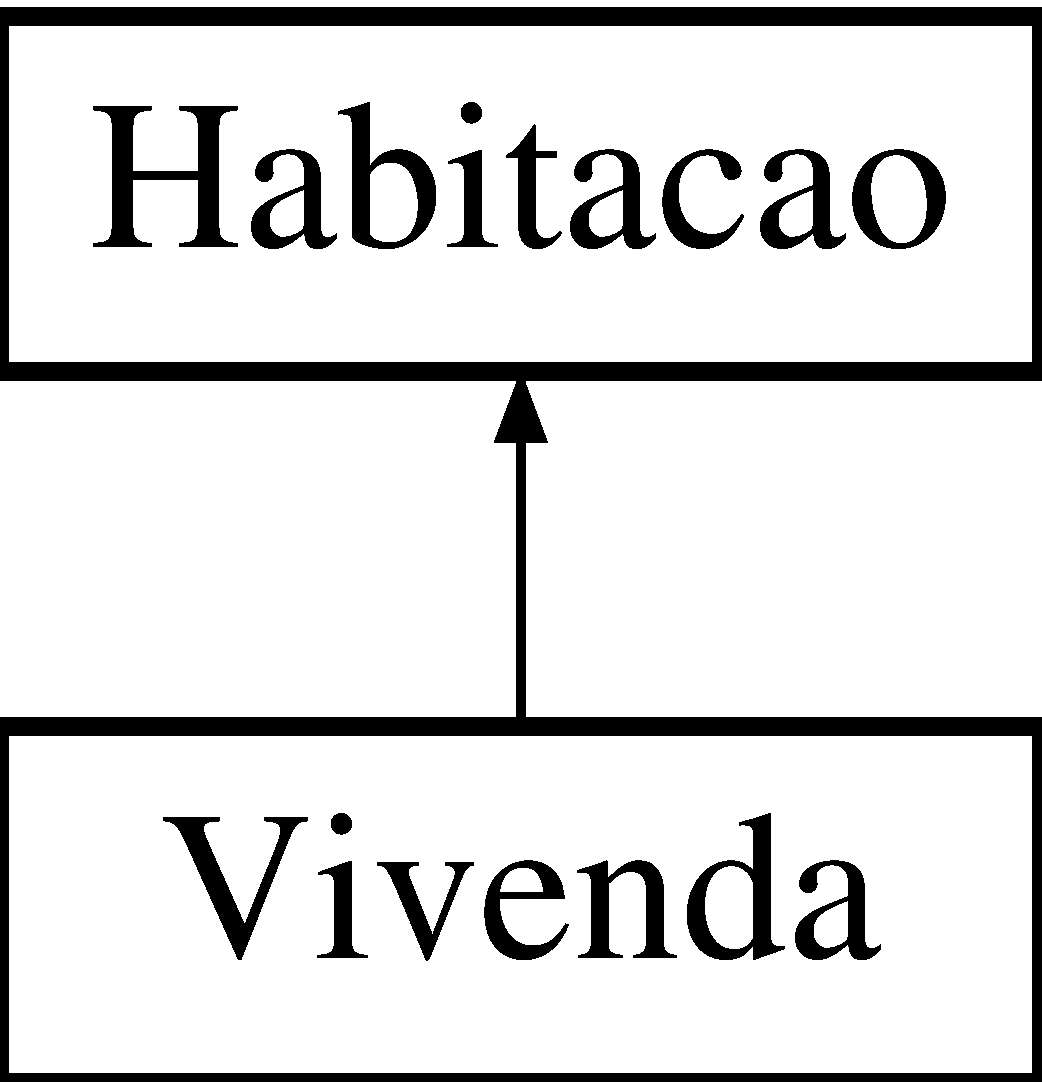
\includegraphics[height=2.000000cm]{class_vivenda}
\end{center}
\end{figure}
\subsection*{Public Member Functions}
\begin{DoxyCompactItemize}
\item 
\hyperlink{class_vivenda_a55423f0f9af77c03237c80a07e9e7509}{Vivenda} (string morada, int area\+Habitacao, int area\+Exterior, bool tem\+Piscina)
\begin{DoxyCompactList}\small\item\em Função que cria uma vivenda. \end{DoxyCompactList}\item 
float \hyperlink{class_vivenda_ad542e2b2f31da8c24b706211efc880d8}{mensalidade} () const 
\begin{DoxyCompactList}\small\item\em Função que calcula o valor da base mensal de condomínio. \end{DoxyCompactList}\item 
int \hyperlink{class_vivenda_a28bc8d025d1fd0da9a49dc73d34165ef}{get\+Area\+Exterior} () const 
\begin{DoxyCompactList}\small\item\em Função para obter a área exterior. \end{DoxyCompactList}\item 
bool \hyperlink{class_vivenda_aa65508502441fffa1efa69e8708ecc85}{get\+Tem\+Piscina} () const 
\begin{DoxyCompactList}\small\item\em Função para verificar se a vivenda tem piscina. \end{DoxyCompactList}\end{DoxyCompactItemize}


\subsection{Constructor \& Destructor Documentation}
\index{Vivenda@{Vivenda}!Vivenda@{Vivenda}}
\index{Vivenda@{Vivenda}!Vivenda@{Vivenda}}
\subsubsection[{Vivenda(string morada, int area\+Habitacao, int area\+Exterior, bool tem\+Piscina)}]{\setlength{\rightskip}{0pt plus 5cm}Vivenda\+::\+Vivenda (
\begin{DoxyParamCaption}
\item[{string}]{morada, }
\item[{int}]{area\+Habitacao, }
\item[{int}]{area\+Exterior, }
\item[{bool}]{tem\+Piscina}
\end{DoxyParamCaption}
)}\hypertarget{class_vivenda_a55423f0f9af77c03237c80a07e9e7509}{}\label{class_vivenda_a55423f0f9af77c03237c80a07e9e7509}


Função que cria uma vivenda. 


\begin{DoxyParams}{Parameters}
{\em morada} & -\/ localização geográfica da vivenda. \\
\hline
{\em area\+Habitacao} & -\/ area habitacional. \\
\hline
{\em area\+Exterior} & -\/ area exterior. \\
\hline
{\em tem\+Piscina} & -\/ caso a vivenda tenha piscina então é verdadeiro, caso contrário é falso. \\
\hline
\end{DoxyParams}


\subsection{Member Function Documentation}
\index{Vivenda@{Vivenda}!get\+Area\+Exterior@{get\+Area\+Exterior}}
\index{get\+Area\+Exterior@{get\+Area\+Exterior}!Vivenda@{Vivenda}}
\subsubsection[{get\+Area\+Exterior() const }]{\setlength{\rightskip}{0pt plus 5cm}int Vivenda\+::get\+Area\+Exterior (
\begin{DoxyParamCaption}
{}
\end{DoxyParamCaption}
) const}\hypertarget{class_vivenda_a28bc8d025d1fd0da9a49dc73d34165ef}{}\label{class_vivenda_a28bc8d025d1fd0da9a49dc73d34165ef}


Função para obter a área exterior. 

\begin{DoxyReturn}{Returns}
Retorna a área exterior. 
\end{DoxyReturn}
\index{Vivenda@{Vivenda}!get\+Tem\+Piscina@{get\+Tem\+Piscina}}
\index{get\+Tem\+Piscina@{get\+Tem\+Piscina}!Vivenda@{Vivenda}}
\subsubsection[{get\+Tem\+Piscina() const }]{\setlength{\rightskip}{0pt plus 5cm}bool Vivenda\+::get\+Tem\+Piscina (
\begin{DoxyParamCaption}
{}
\end{DoxyParamCaption}
) const}\hypertarget{class_vivenda_aa65508502441fffa1efa69e8708ecc85}{}\label{class_vivenda_aa65508502441fffa1efa69e8708ecc85}


Função para verificar se a vivenda tem piscina. 

\begin{DoxyReturn}{Returns}
Retorna verdade se a vivenda tem piscina e falso caso contrário. 
\end{DoxyReturn}
\index{Vivenda@{Vivenda}!mensalidade@{mensalidade}}
\index{mensalidade@{mensalidade}!Vivenda@{Vivenda}}
\subsubsection[{mensalidade() const }]{\setlength{\rightskip}{0pt plus 5cm}float Vivenda\+::mensalidade (
\begin{DoxyParamCaption}
{}
\end{DoxyParamCaption}
) const\hspace{0.3cm}{\ttfamily [virtual]}}\hypertarget{class_vivenda_ad542e2b2f31da8c24b706211efc880d8}{}\label{class_vivenda_ad542e2b2f31da8c24b706211efc880d8}


Função que calcula o valor da base mensal de condomínio. 

\begin{DoxyReturn}{Returns}
Retorna o valor da base mensal de condomínio. 
\end{DoxyReturn}


Reimplemented from \hyperlink{class_habitacao_a479d2307661c87b05242b86ba849fb6e}{Habitacao}.



The documentation for this class was generated from the following files\+:\begin{DoxyCompactItemize}
\item 
Vivenda.\+h\item 
Vivenda.\+cpp\end{DoxyCompactItemize}

%--- End generated contents ---

% Index
\backmatter
\newpage
\phantomsection
\clearemptydoublepage
\addcontentsline{toc}{chapter}{Index}
\printindex

\end{document}
